\documentclass{article}

% if you need to pass options to natbib, use, e.g.:
%     \PassOptionsToPackage{numbers, compress}{natbib}
% before loading neurips_2018

% ready for submission
% \usepackage{neurips_2018}

% to compile a preprint version, e.g., for submission to arXiv, add add the
% [preprint] option:
%     \usepackage[preprint]{neurips_2018}

% to compile a camera-ready version, add the [final] option, e.g.:
\usepackage[final]{neurips_2018}

% to avoid loading the natbib package, add option nonatbib:
%     \usepackage[nonatbib]{neurips_2018}

\usepackage[utf8]{inputenc} % allow utf-8 input
\usepackage[T1]{fontenc}    % use 8-bit T1 fonts
\usepackage{hyperref}       % hyperlinks
\usepackage{url}            % simple URL typesetting
\usepackage{booktabs}       % professional-quality tables
\usepackage{amsfonts}       % blackboard math symbols
\usepackage{nicefrac}       % compact symbols for 1/2, etc.
\usepackage{microtype}      % microtypography
\usepackage{graphicx}
\usepackage{bbm}
\usepackage{amssymb}
\usepackage{listings}
\usepackage{float}
\usepackage{amsmath}        % multilines equation + DeclareMathOperator
\usepackage[options]{algorithm2e}

\newcommand{\softmax}{\mathrm{softmax}}
\newcommand{\sigmoid}{\mathrm{sigmoid}}
\DeclareMathOperator*{\argmax}{arg\,max}
\DeclareMathOperator*{\argmin}{arg\,min}




\title{Boosting many low capacity classifiers compared to boosting fewer high capacity classifiers in a context of multi-class classification}

% The \author macro works with any number of authors. There are two commands
% used to separate the names and addresses of multiple authors: \And and \AND.
%
% Using \And between authors leaves it to LaTeX to determine where to break the
% lines. Using \AND forces a line break at that point. So, if LaTeX puts 3 of 4
% authors names on the first line, and the last on the second line, try using
% \AND instead of \And before the third author name.

\author{%
 Jonathan Guymont, Marzieh Mehdizad, L\'ea Ricard,\\ \textbf{Jeff Sylvestre Decary \& Joseph D. Viviano}\\
  Department of Computer Science\\
  Universit\'e de Montr\'eal\\
  \texttt{jonathan.guymont@umontreal.ca}, \texttt{marzieh.mehdizadeh@gmail.com}, \texttt{lea.ricard@umontreal.ca},\\
  \texttt{jeff.sylvestre-decary@polymtl.ca}, \texttt{joseph@viviano.ca} \\
}

\begin{document}
% \nipsfinalcopy is no longer used

\maketitle
\section{Introduction}
Boosting is a method for improving the performance of a learning algorithm by combining weak learners, each of them having to perform just better than random \cite{Schwenk}. \textit{AdaBoost}\cite{Freund} is a state-of-the-art boosting algorithm known for being robust to overfitting. Many empirical studies using decision trees have shown impressive results \cite{Schwenk} and few papers have experiment boosting neural networks with success.

We want to investigate whether the primary benefit of boosting comes from simply increasing the total capacity of the ensemble, or whether boosting is an inherently better learning algorithm than using a single powerful model. To do this, we propose to compare models in the same family where we reduce the capacity of the model and increase the number of boosted models such that all ensembles have approximately the same number of trainable parameters. We hypothesize that using more learners with lower individual capacity will outperform a single learners with equivalent capacity.

We tested this hypothesis in the context of two multi-class classification tasks. The three model families we compare are Decision Trees, Logistic Regression and Multi-layer Perceptron (MLP). All boosted ensembles were created with Adaboost. The capacity of Logistic Regression was not controlled and will serve as our baseline.  

\section{Algorithms}

\subsection{Logistic regression}
Logistic regression is a simple supervised learning classifier. This linear classifier is a generalized linear model (GLM) defined by 
\begin{equation}
    \ln \frac{p(y=1|x)}{1-p(y=1|x)}= b_0+b_1x_1+...+b_j x_j
\end{equation}
which can be rearrange to 
\begin{equation}
    p(y=1|x)=\frac{1}{1+e^{-(b_0+b_1x_1+...+b_j x_j)}}=\sigmoid(b_0+b_1x_1+...+b_j x_j)
\end{equation}
The output of this last function tells us the probability of being in class 1 or in class 2 ($p(y=2|x)=1-p(y=1|x)$) and the predicted class will be the one with the highest probability. This simple classifier can be seen as an Multi-layer perceptron without hidden layer, because we modify the weight of every input in a way that we minimize our error. 

%\begin{figure}[H]
%    \centering
%    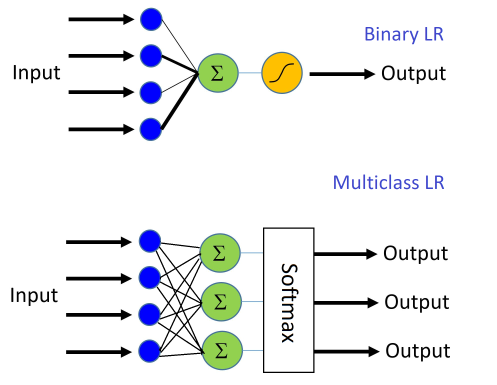
\includegraphics[scale=.6]{Figures/LR.png}
%    \caption{Logistic Regression}
%    \label{fig:LR}
%\end{figure}

We will be working with mutliclass data sets, and, as describe in Figure 1, multiclass logistic regression use softmax function 
\[
    p(y=k|X) = \frac{e^{(b_{0}+b_{1}x_{1}+...+b_{j} x_j)}}{\sum_{i=1}^me^{(b_{0}+b_{1}x_{1}+...+b_{j}x_j)}}
\]
to determine the probability of being in a specific class. To determine the predicted class, we will usually take the $\argmax$ of the probability computed for all classes. This represent only a transformation of the binary logistic regression.

\subsection{Decision tree} Decision tree are non-parametric supervised algorithm that can be used for classification. They are binary tree with a \texttt{if else} rule at each node indicating whether the right or the left edge should be followed. 

Let $d$ be the number of features. At a particular node of the tree, $\sqrt{d}$ features were randomly selected to be tested. Then the model select the pair \emph{(feature, rule)} for which the KL-divergence of the prior distribution $p(D_m)$ from the posterior distribution $p(D_m|\theta_m)$ is maximized, where $D_m$ is the set of samples at node $m$ and $\theta_m$ is a splitting rule at node $m$. Formally, given the empirical expected value of the log-likelihood of the prior at a node $m$
\begin{equation}
    H(D_m)=\sum_{k=1}^K p(y_i = k | x_i \in D_m) \log p(y_i = k | x_i \in D_m)
\end{equation}
and the posterior log-likelihood given a rule splitting rule $\theta_m$
\begin{align}
    H(D_m|\theta_m)
    =&p(x\in D_{m+1})\sum_{k=1}^K p(y_i = k | x\in D_{m+1}) \log p(y_i = k | x\in D_{m+1}) \\
    ~~+&~ p(x\in D_{m+2})\sum_{k=1}^K p(y_i = k | x\in D_{m+2}) \log p(y_i = k | x\in D_{m+2}) 
\end{align}
- where $D_{m+1}$ represent the samples going to the left child and $D_{m+2}$ represents the samples going to the right child under the rule $\theta_m$- we will select the rule $\theta_m$ such that
\begin{equation}
    \theta_m = \argmax_{\theta} H(D_m)-H(D_m|\theta).
\end{equation}
Note that since the entropy of the prior is constant, this is equivalent has selecting the rule that minimize the negative log-likelihood.

Each node is divided in two child until either the maximal depth of the tree $\mathcal{T}$ is reached or the minimum number of sample at a node $\min_{sample}$ is reached. $\mathcal{T}$ and $\min_{sample}$ are two hyperparameters that we used to control the capacity. The software that we used did not support \emph{pruning} so these two parameters were also our only mean of regularization. 

\subsection{Multi-layer perceptron} 
Multi-layer perceptron (MLP) is a supervised learning algorithm which can be use for classification and regression problem, and can learn complex decision boundaries to correctly classify non-linearly separable data. MLP has an architecture with at least three layers where the first layer is the input (training data sets) and the last layer is the output. The in-between layers are called hidden layers, each usually implementing an non-linearity via an activation function, such as a logistic function or rectified linear unit (ReLU).\\

%\begin{figure}[H]
%    \centering
%    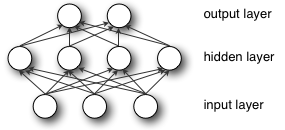
\includegraphics[scale=.8]{Figures/mlp.png}
%    \caption{Multi-layer perceptron}
%    \label{fig:MLP}
%\end{figure}

MLP training consists of forward propogation of some inputs through the weight matrices and their bias terms to produce predictions. Eq. \ref{eq:mlp} describe a MLP with one hidden layer with a sigmoid activation function $\sigma(.)$:
\begin{equation}
    \begin{split}
        \mathbf{h} =& \sigma(\mathbf{W}^{(1)}\mathbf{x} + \mathbf{b}^{(1)})\\
        \mathbf{y} =& \softmax(\mathbf{W}^{(2)}\mathbf{h} + \mathbf{b}^{(2)})\\
        c =& \argmax \mathbf{y} 
    \end{split}
    \label{eq:mlp}
\end{equation}

%\begin{algorithm}[H]
%\SetAlgoLined
% Given: $(x_1,y_1),...,(x_m,y_m)$ where $x_i \in \mathcal{R}^k$, $y_i \in Y$\\
% Initialize $w^{(1)}\in \mathcal{R}^{k\times n}$ and $b^{(1)} \in \mathcal{R}^n$\;
% Initialize $w^{(2)}\in \mathcal{R}^{k\times z}$ and $b^{(2)} \in \mathcal{R}^z$\;
% \For{$t=1,...,m$}{
% Compute the output vectors for each n neurons: $h^s$=$w^{(1)}^Tx^{(t)}+b^{(1)}$\\
% Compute the activation function on each output vectors: $h^a=\sigma(h^s)$\\
% Compute the output vectors for each z class: $o^s=w^{(2)}^Th^{a}+b^{(1)}$ \\
% Compute the activation function for each z class: $o^a= \psi(o^s)$\\
% The prediction could be: \argmax(o^a)\\
% }
% \caption{Multi-layer perceptron forward propagation}
%\end{algorithm}

The loss of the prediction $c$ is then backpropagated through the network to find new weights and biases which minimize the error made by the MLP via gradient descent. Specifically, one finds the find the derivative of the negative log-likelihood of the predicted class with respect to all weights and bias using the chain rule. We will refer the interested reader to \cite{Pin} to find a complete description of the backpropagation algorithm.

An MLP of arbitrary width can be used to express any continuous function, making MLP a strong classifier.

\subsection{Adaboost}

Adaboost was created to provide a way of building a strong classifier composed of multiple weak classifiers. This algorithm trains each weak classifier sequentially, with each new weak learner giving more weight to examples in the training set that previous learners incorrectly classified. The idea behind this algorithm is that training examples which are harder to classify correctly should give us more information regarding the optimal classifier\cite{Zha}. By increasing the weight of a misclassified points and decreasing the weight of well classified points, Adaboost makes sure that each weak classifier introduced will do it's best to minimize the ensemble error. The complete Adaboost algorithm is the following:

\begin{algorithm}[H]
\SetAlgoLined
 Given: $(x_1,y_1),...,(x_m,y_m)$ where $x_i \in X$, $y_i \in Y$\\
 Initialize $D_1(i)=1/m$\;
 \For{$t=1,...,T$}{
  Train weak learner using distribution $D_t$.\\
  Get weak classifier $h_t$ : $X$ $\rightarrow{\mathbf{R}}$.\\
  Choose $\alpha_t \in \mathbf{R}$.\\
  Update: $D_{t+1}(i) = \frac{D_t(i)\exp(-\alpha_t y_i h_t(x_i))}{Z_t}$.
  }
 \caption{Adaboost}
\end{algorithm}

\section{Methodology}

\subsection{Data} 
We experimented on two different classification tasks from two different data sets

\begin{itemize}
    \item Wine Quality: Using a joint data set of red and white Portuguese wines, predict whether these wines are rated by experts from poor to excellent (score between 0 and 10).
    \item Balanced\footnote{We randomly selected 2700 instances of each class to have the biggest possible balanced data set.} Forest Cover Type: Using cartographic variables, predict whether these features correspond to which of the 7 forest cover type (7 class classification).  
\end{itemize}

These two data sets present interesting features and very different size. The Wine data set has 4898 instances with 12 attributes compared to 18\ 900 instances (selected over a total of 581\ 012 instances) with 54 attributes for the Forest Cover Type set. All the attributes of the Wine data set are real values, while the Forest Cover Type set has 44 binary (describing the soil type and the wilderness area) and 10 real values attributes. These two very different data sets will give us an opportunity to experiment on whether the data sets has many instances and attributes or not.

In both data sets, the data was normalized before training. For the wine quality data set, some classes were merged together since the quantity of examples with extreme quality was too small (see Appendix \ref{Appendice_Wine}). Specifically, class 3 was merged to class 4 and class 9 was merged to class 8.

The data set were split into a training and a test set with a proportion of 85\% and 15\% respectively.

\subsection{Hyper-parameter search}
We used the training set to learn the parameters of the model and the validation set to do hyper-parameter selection using randomized search \cite{Berg} with 50 iterations, and 10 fold inner-loop cross validation (these folds were applied to the training data only). This procedure was performed in the context of outer 10-fold stratified cross validation to find the model with the best average accuracy across all folds. Empirical risk was estimated at the end of training by generating predictions with the best model on the test set. 

For the decision tree, capactiy was controlled via the maximum allowed tree depth. The maximum depth for the single (not boosted) classifier was selected among $[6, 7,...,12]$ for the wine quality experiment and $[11, 12, ..., 20]$ for the Forest Cover Type. The maximum depth was search among different set because the cover type dataset contains significantly more features then the wine quality dataset. The constraint for the minimum number of samples required to split an internal node in two leaves was chosen among the set $[2, 3, ... \lfloor 0.01\cdot |D_n|\rfloor]$. The constraint for the minimum number of samples at a node was chosen among $[1, 2, ... \lfloor 0.005\cdot |D_n|\rfloor]$.

For the logistic regression, the regularization parameter $C$ was selected among the interval $[0.001, 10]$.

For the MLP, capacity was controlled via the size of the hidden layer. The maximum hidden layer size for the single (not boosted) classifier was selected in the range $[100, 300]$ for both datasets. We additionally searched for the initial learning rate uniformly from a logarithmic normal distribution between $[10^{-6}, 10^{-1}]$ and the L2 penalty uniformly from a logarithmic normal distribution between $[10^{-6}, 10^{-1}]$. All models were parametrized with ReLU activation functions, optimized via stochastic gradient descent using nesterov's momentum parameter of 0.9, learning rate decay every 10 epochs by dividing the learning rate by 10, early stopping, and a batch size of 32.

For all boosted models, the learning rate of adaboost was found using randomized cross validation searching for the learning rate uniformly between $[10^{-5}, 10^{-1}]$.

\subsection{Performance evaluation}
Because the wine dataset was unbalanced (i.e. the number of instances per class is highly unequal), we chose to use $F_1$ score both for hyperparameter tuning and reporting our test scores. We didn't use classification accuracy for the experiments since they would be functionally similar for the balanced Forest Cover Type dataset, and likely over-optimistic for the unbalanced Wine dataset.

\subsubsection{$F_1$ score}
The performance metric used is the $F_1$ score, a weighted average of the precision and the recall. The precision is the the number of true positives divided by the sum of true positives and false positives. It can be interpreted as the classifier exactness. The recall is the number of true positives divided by the number of true positives and the number of false negatives. It can be interpreted as the classifier completeness.

%Check if we should keep this part (enough space?)
In the case of a multi-class classification, the overall $F_1$ score is the unweighted average of the $F_1$ score of each class. This was done to give more weight to the under-represented classes. True positives, false positives and false negatives of a class $y_k$ are defined as:
\begin{itemize}
    \item True positives: Examples that are correctly predicted as $y_k$ ;
    \item False positives: Examples that are incorrectly predicted as $y_k$;
    \item False negatives: Examples that are incorrectly predicted as $y_i$, when the correct class is $y_k$.
\end{itemize}

\subsection{Capacity variation}
To test our hypothesis, we had to decrease the capacity of decision tree and MLP model while proportionally-increasing the number of classifiers. 

For decision tree, we vary the capacity of the model by varying the maximum depth of the tree (and consequently the number of nodes). A deeper tree is more expressive, thus smaller tree were paired with high number of classifiers. More specifically, we were trying to maintain the number of node about constant. When we decreased the depth of the tree by 1, we doubled the number of classifiers, since removing one layer in a balanced binary tree removes about half the nodes. Note that we didn't not control the number of nodes; more investigation would be necessary to make sure the number of nodes was actually constant.

For the MLP, we vary the capacity of the model by modifying the number of hidden units in the network, and therefore the number of weights trained. A MLP with more hidden units is able to express more complicated hyperplanes, thus smaller MLPs were boosted proportionally to keep the number of trained parameters roughly constant. This was done by dividing the initial hidden layer size found via cross validation by the number of requested boosters.

\section{Results}
Tables \ref{table:Results_Wine} and \ref{Table:Results_Forest} show a summary of the performance (accuracy and $F_1$ score) of the different boosted models on the Wine Quality and the Forest Cover Type datasets. The pair of parameters used is \textit{(value of hyper-parameter controlling capacity, number of classifiers)}. For the Logistic Regression, the capacity does not vary. For the Decision Tree model, the hyper-parameter controlling the capacity is the maximum depth of the tree, while it's the number of neurons for the MLP. 

Without explicitly changing the capacity, the $F_1$ score of the Logistic Regression model improves when the number of classifiers feed into \textit{AdaBoost} increases, both for Wine Quality and Forest Cover Type datasets.

 Figure \ref{fig:Tree_results} in Appendix \ref{Appendice_Tree} show the $F_1$ score for the different pair \emph{(maximum depth, number of classifiers)} for the decision tree model. Figure \ref{fig:Tree_results} a) and b) show that the $F_1$ score is relatively constant for both the Wine Quality classification and the cover type experiment. We also note that for the smaller tree (maximum depth of 6 or less) the performance is decreasing significantly in the Cover Type experiment. We suspect that this is due to the large number of features in the Cover Type dataset. This result tells us that increasing the number of classifiers balanced out the loss of capacity caused by decreasing the depth of the trees. We also note that our method for maintaining the number of parameters constant does not guarantee that the number of nodes is constant after adding a proportional number of boosters. Further investigation of the distribution of the number of nodes across models would be required to conclude that there is no value in boosting when the total number of parameters in maintained constant.

Figure \ref{fig:MLP_results} in Appendix \ref{Appendice_MLP} show the $F_1$ score on the training and test set of boosted classifiers using MLP. For both datasets, boosting appears to approximately balance out the effect of reducing capacity for all combinations tested. When reducing capacity without boosting, we found performance decreases, confirming that adding more learners via Adaboost offsets the loss of individual-model capacity. See Appendix \ref{Appendix_NoBoosting} for the non-boosted results.

\begin{table}[h!]
\label{table:Results_Wine}
\caption {Test performance of models on boosted Wine Quality data set} \label{fig:results}
\begin{center}
\begin{tabular}{|l|l|l|l|l|l|l|}
    \hline
    \multicolumn{7}{|c|}{Wine Quality (boosted)}\\
    \hline
    &\multicolumn{2}{|c|}{Best result}&\multicolumn{2}{|c|}{Many weak learners}&\multicolumn{2}{|c|}{Few stronger learners}\\
    \hline
    Model & Param. & $F_1$ & Param. & $F_1$ & Param. & $F_1$ \\
    \hline \hline
     LR & (-,10) & 0.36 & (-,20) & 0.36 & (-,1) & 0.26 \\
     Dec. Tree & (6,4) & 0.34 & (1,128) & 0.32 & (8,1) & 0.32 \\
     MLP  & (133,2) & 0.35 & (13,20) & 0.34 & (267,1) & 0.35 \\
     \hline
\end{tabular}
\end{center}
\end{table}

\begin{table}[h!]
\label{Table:Results_Forest}
\caption {Test performance of models on boosted Forest Cover Type data set} \label{fig:results}
\begin{center}
\begin{tabular}{|l|l|l|l|l|l|l|}
    \hline
    \multicolumn{7}{|c|}{Forest Cover Type (boosted)}\\
    \hline
    &\multicolumn{2}{|c|}{Best result}&\multicolumn{2}{|c|}{Many weak learners}&\multicolumn{2}{|c|}{Few stronger learners}\\
    \hline
    Model & Param. & $F_1$ & Param. & $F_1$ & Param. & $F_1$ \\
    \hline \hline
     LR & (-,10) & 0.43 & (-,20) & 0.42 & (-,1) & 0.29 \\
     Dec. Tree & (11,64) & 0.53 & (10,128) & 0.51 & (17,1) & 0.41 \\
     MLP  & (91,2) & 0.74 & (9,20) & 0.70 & (182,1) & 0.74 \\
     \hline
\end{tabular}
\end{center}
\end{table}


\section{Discussion and conclusion}

In conclusion, it appears that model capacity is the primary driver of classification results. In the absence of boosting, reducing model capacity decreases performance, as expected. After proportionally adding additional boosted classifiers to balance out the loss of per-model capacity, we recover the original performance of the model, but fail to meaningfully surpass it. Therefore, we can conclude that having a smaller number of models with high capacity preform approximately equally to a larger number of models with proportionally smaller capacity. In a few cases, performance drops when the capacity of the weak classifiers is too small (see the lowest capacity MLP models).

Model performance was not 100\% stable run-to-run. Given more available computation time, we would have liked to repeat all experiments 10-100 times to obtain good confidence intervals on the $F_1$ scores reported for each ensemble. This would allow us to more meaningfully state that there is no difference in the performance of the differently-boosted models.

\textit{AdaBoost} performance degrades in presence of noise \cite{Diet}. The poor performance of our boosted models on the Wine Quality dataset (less than a $F_1$ score of 40\%) might be related to label noise, as wine ratings are highly subjective. Dietterich \cite{Diet} reported that bagging is more appropriate for noisy classification. We propose a follow up experiment comparing bagging and boosting methods for datasets with noisy labels.

Secondly, we question whether we should have combined the red and white wine datasets for the wine quality task. While both datasets used the same features, we believe that experts might rank particular features of good white wine very differently than features of good red wine. In retrospect, we would have been better off either training and testing the two datasets separately, or adding a binary feature denoting wine type (white vs. red). We predict that the decision tree classifier in particular would have benefited from this additional feature, and quite possibly for the MLP classifier. We predict that the logistic regression classifier would only benefit strongly from splitting the dataset into two.


\newpage
\begin{thebibliography}{99}

\bibitem{Berg} Bergstra, J., & Bengio, Y. (2012). Random search for hyper-parameter optimization. Journal of Machine Learning Research, 13(Feb), 281-305.

\bibitem{Gar} García, E., & Lozano, F. (2007, July). Boosting Support Vector Machines. In MLDM Posters (pp. 153-167).

\bibitem{Zha} Zhang, H., & Gu, C. (2008). Support vector machines versus Boosting. Electrical Engineering UC, Berkeley, 1-19.

\bibitem{Pin} Pineault, J. (2018). Neural networks slides. Computer science, Mcgill University.

\bibitem{Schwenk}Schwenk, H. and Bengio, Y. (2000). Boosting Neural Networks. Neural Comput. 12, 8, 1869-1887. 

\bibitem{Freund} Freund, Y. (1995). Boosting a weak learning algorithm by majority. Information and computation, 121(2):256-285.

\bibitem{Diet} Dietterich, T. (2000). An Experimental Comparison of Three Methods for Constructing Ensembles of Decision Trees: Bagging, Boosting, and Randomization. Mach. Learn.. 40. 10.1023/A:1007607513941. 

\bibitem{Singh} Singh, A. (2010). Can we make dumb learners smart? Mach. Learn.. Carnegie Mellon University


\end{thebibliography}


%-----------------------------------------------------
%
%                   Appendices
%
%----------------------------------------------------

\newpage
\appendix

\section{Logistic regression results}
\label{Appendice_LR}

\begin{figure} [H]
    \centering
    \begin{tabular}{cccc}
    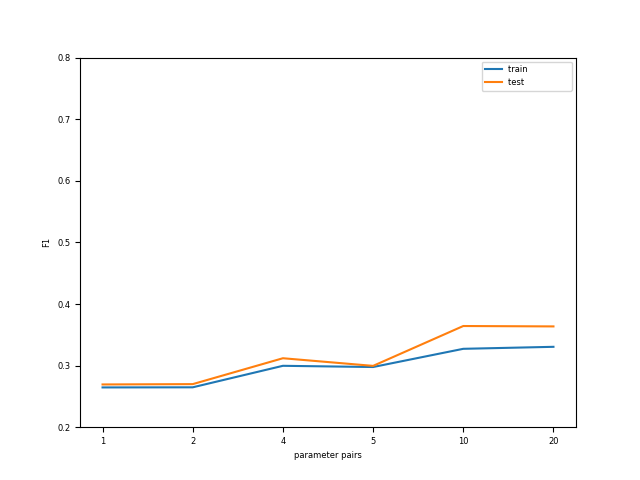
\includegraphics[width=0.9\textwidth]{Results_LR/lr-wine-boosted_f1.png}\\
    (a) \\[6pt]
    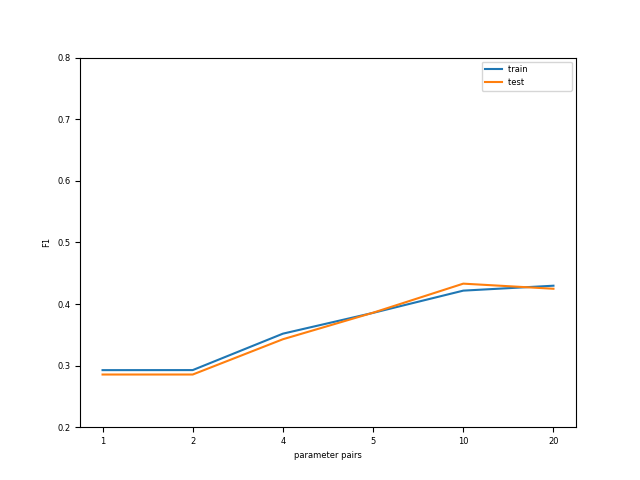
\includegraphics[width=0.9\textwidth]{Results_LR/lr-covtype-boosted_f1.png}\\ (b)  \\[6pt]
    \end{tabular}
    \caption{Performance on test and training set by parameter pairs (tree maximum depth, number of tree boosted) on (a) Wine Quality data and (b) Forest Cover Type boosted with Decision Tree classifiers}
    \label{fig:Tree_results}
\end{figure}


\section{Decision tree results}
\label{Appendice_Tree}

\begin{figure} [H]
    \centering
    \begin{tabular}{cccc}
    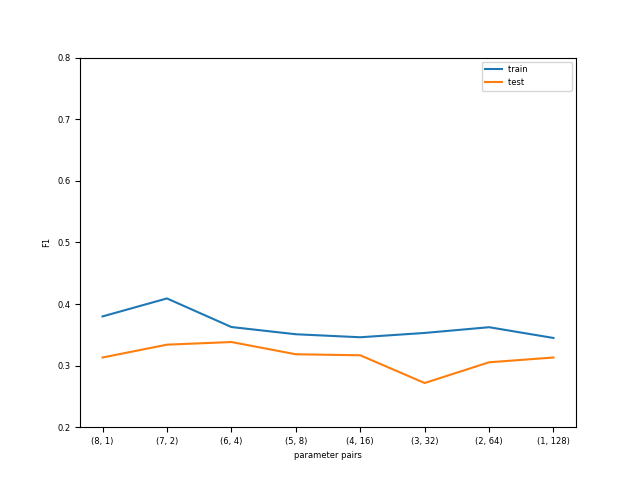
\includegraphics[width=0.9\textwidth]{Results_Tree/tree-wine-boosted_f1.png}\\
    (a) \\[6pt]
    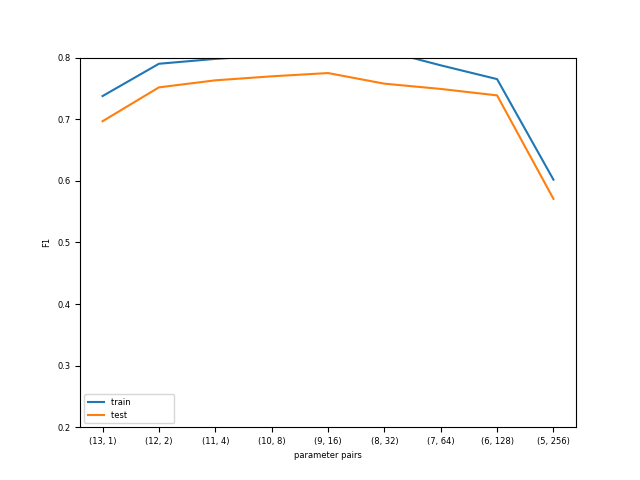
\includegraphics[width=0.9\textwidth]{Results_Tree/tree-covtype_balanced-boosted_f1.png}\\ (b)  \\[6pt]
    \end{tabular}
    \caption{Performance on test and training set by parameter pairs (tree maximum depth, number of tree boosted) on (a) Wine Quality data and (b) Forest Cover Type boosted with Decision Tree classifiers}
    \label{fig:Tree_results}
\end{figure}

\section{MLP results}
\label{Appendice_MLP}

\begin{figure} [H]
    \centering
    \begin{tabular}{cccc}
    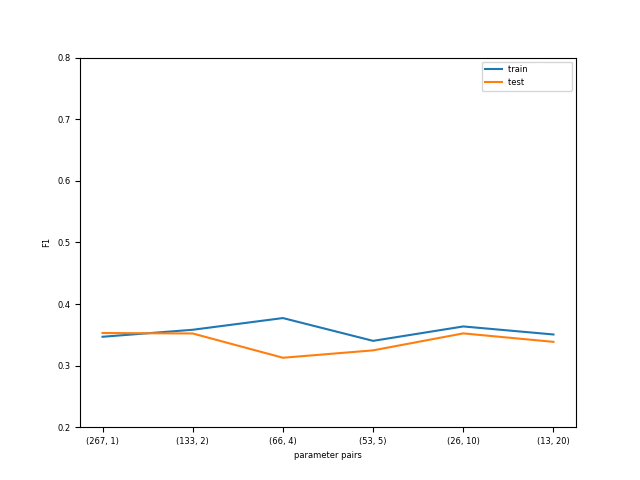
\includegraphics[width=0.9\textwidth]{Results_MLP/mlp-wine-boosted_f1.png}\\
    (a) \\[6pt]
    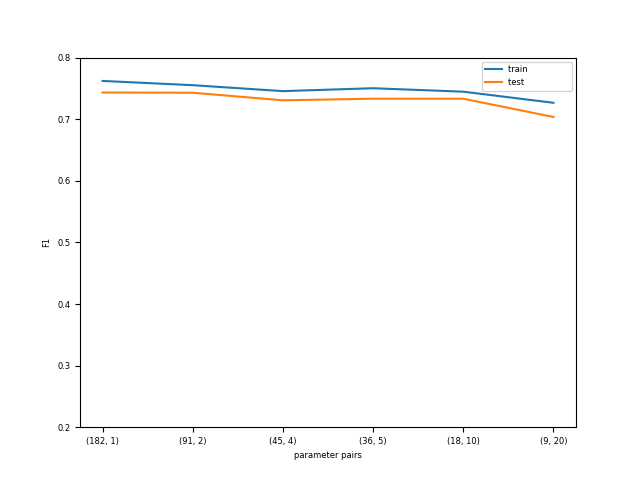
\includegraphics[width=0.9\textwidth]{Results_MLP/mlp-covtype_balanced-boosted_f1.png}\\ (b)  \\[6pt]
    \end{tabular}
    \caption{Performance on test and training set by parameter pairs (number of neurons, number of MLP boosted) on (a) Wine Quality data and (b) Forest Cover Type boosted with MLP classifiers}
    \label{fig:Tree_results}
\end{figure}

\section{Effect of capacity reduction in the absence of boosting}
\label{Appendix_NoBoosting}

\begin{figure} [H]
    \centering
    \begin{tabular}{cccc}
    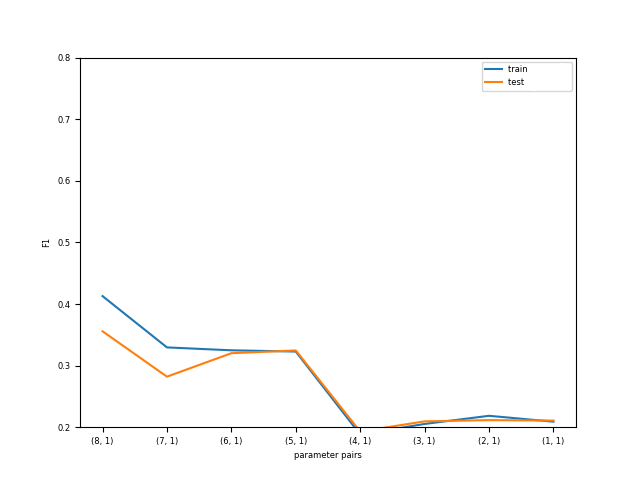
\includegraphics[width=0.9\textwidth]{Results_Tree/tree-wine-not-boosted_f1.png} \\
    (a)\\[6pt]
    \end{tabular}
    \begin{tabular}{cccc}
    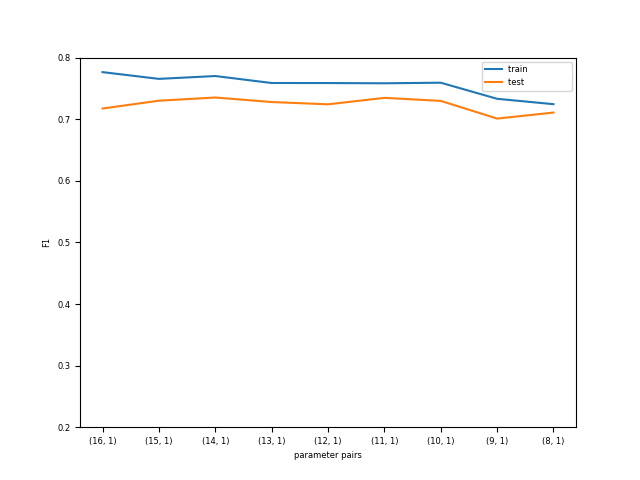
\includegraphics[width=0.9\textwidth]{Results_Tree/tree-covtype_balanced-not-boosted_f1.png} \\
    (b)\\[6pt]
    \end{tabular}
\end{figure}
\begin{figure}[H]\ContinuedFloat
    \begin{tabular}{cccc}
    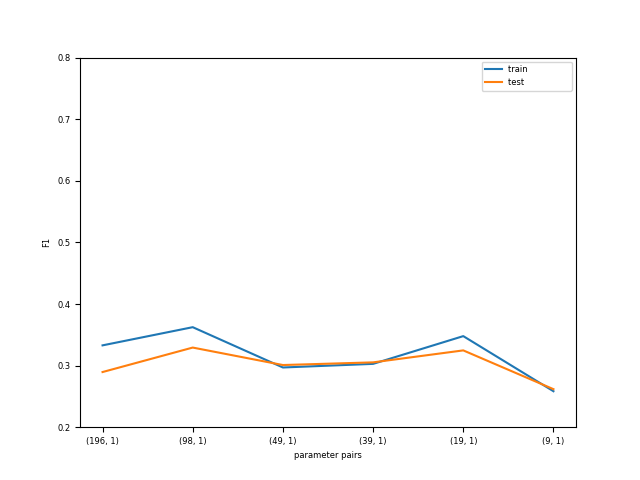
\includegraphics[width=0.9\textwidth]{Results_MLP/mlp-wine-not-boosted_f1.png} \\
    (c)\\[6pt]
    \end{tabular}
    \begin{tabular}{cccc}
    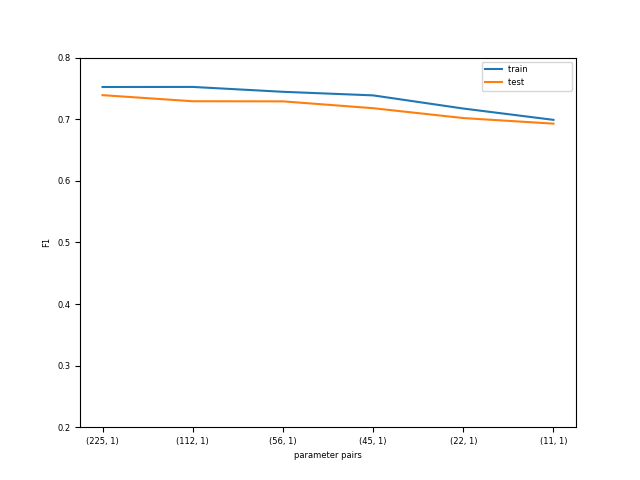
\includegraphics[width=0.9\textwidth]{Results_MLP/mlp-covtype_balanced-not-boosted_f1.png} \\
    (d)\\[6pt]
    \end{tabular}
    \caption{Effect of capacity reduction in the absence of boosting for (a) Decision Tree on Wine Quality, (b) Decision Tree on Forest Cover Type, (c) MLP on Wine Quality and (d) MLP on Forest Cover Type.}
    \label{fig:MLP_results}
\end{figure}


\section{Wine quality dataset analysis}
\label{Appendice_Wine}
% \begin{figure} [H]
% \centering
%     \begin{tabular}{cccc}
%     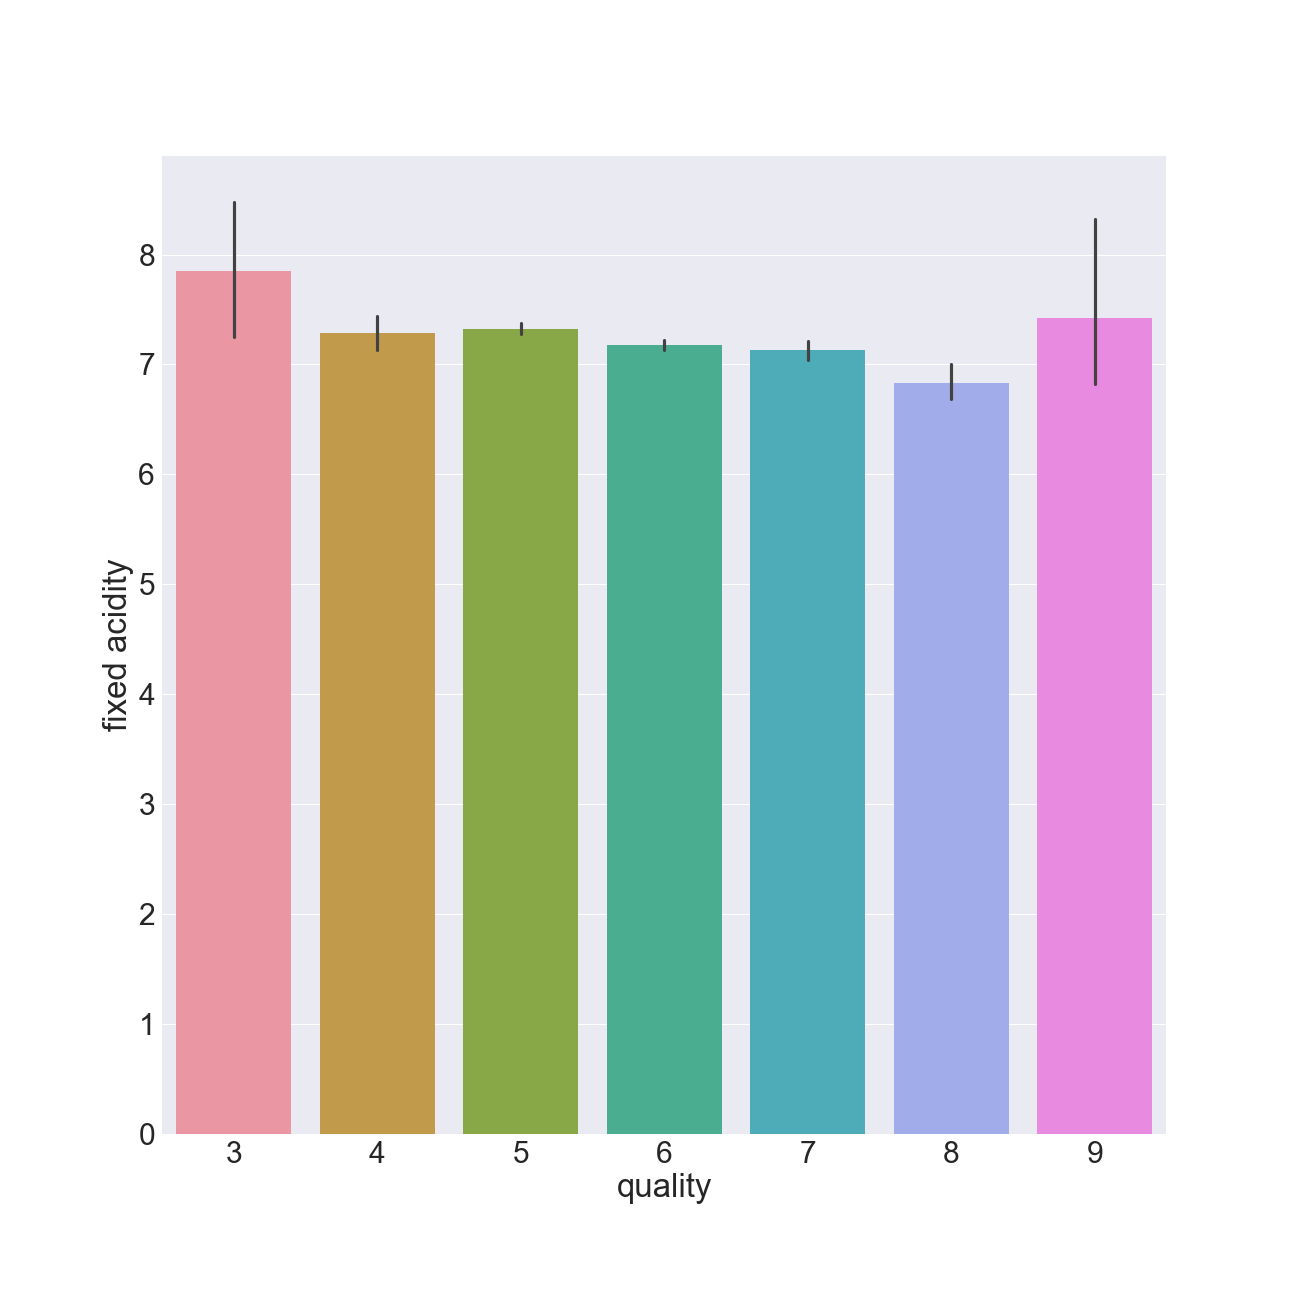
\includegraphics[width=0.5\textwidth]{Figures/fixed_acidity_plot.png} &
%     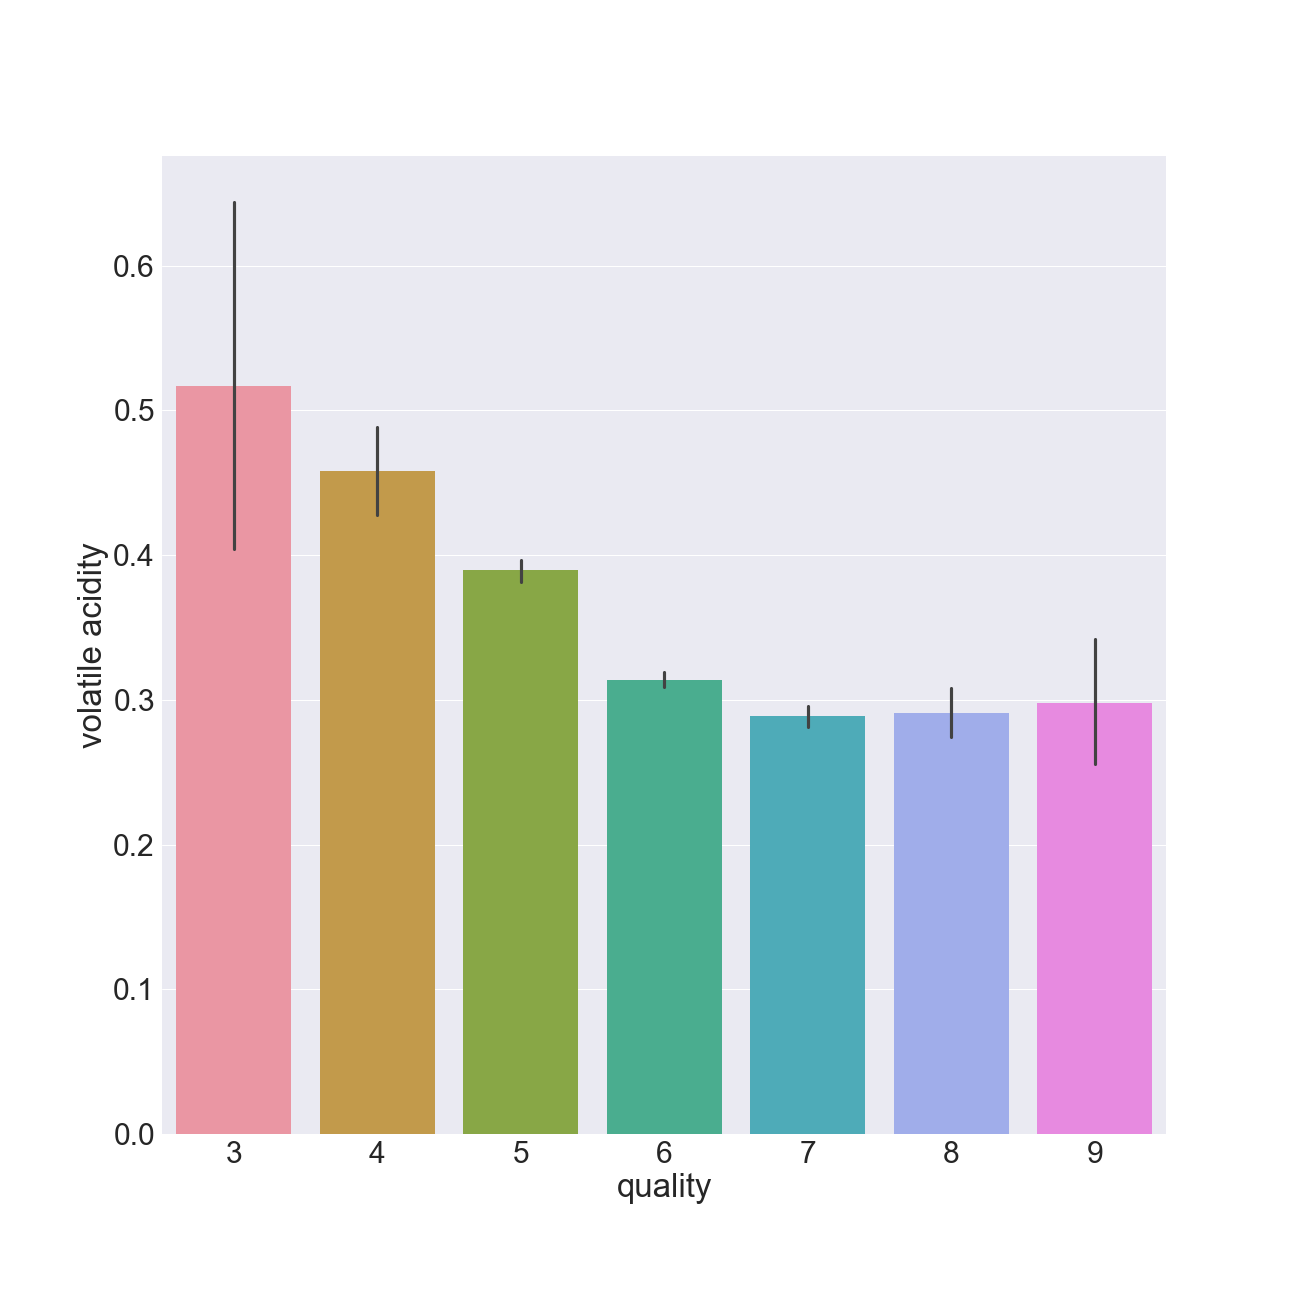
\includegraphics[width=0.5\textwidth]{Figures/volatile_acidity_plot.png}  \\
%     (a)  & (b) \\[6pt]
%     \end{tabular}
%     \begin{tabular}{cccc}
%     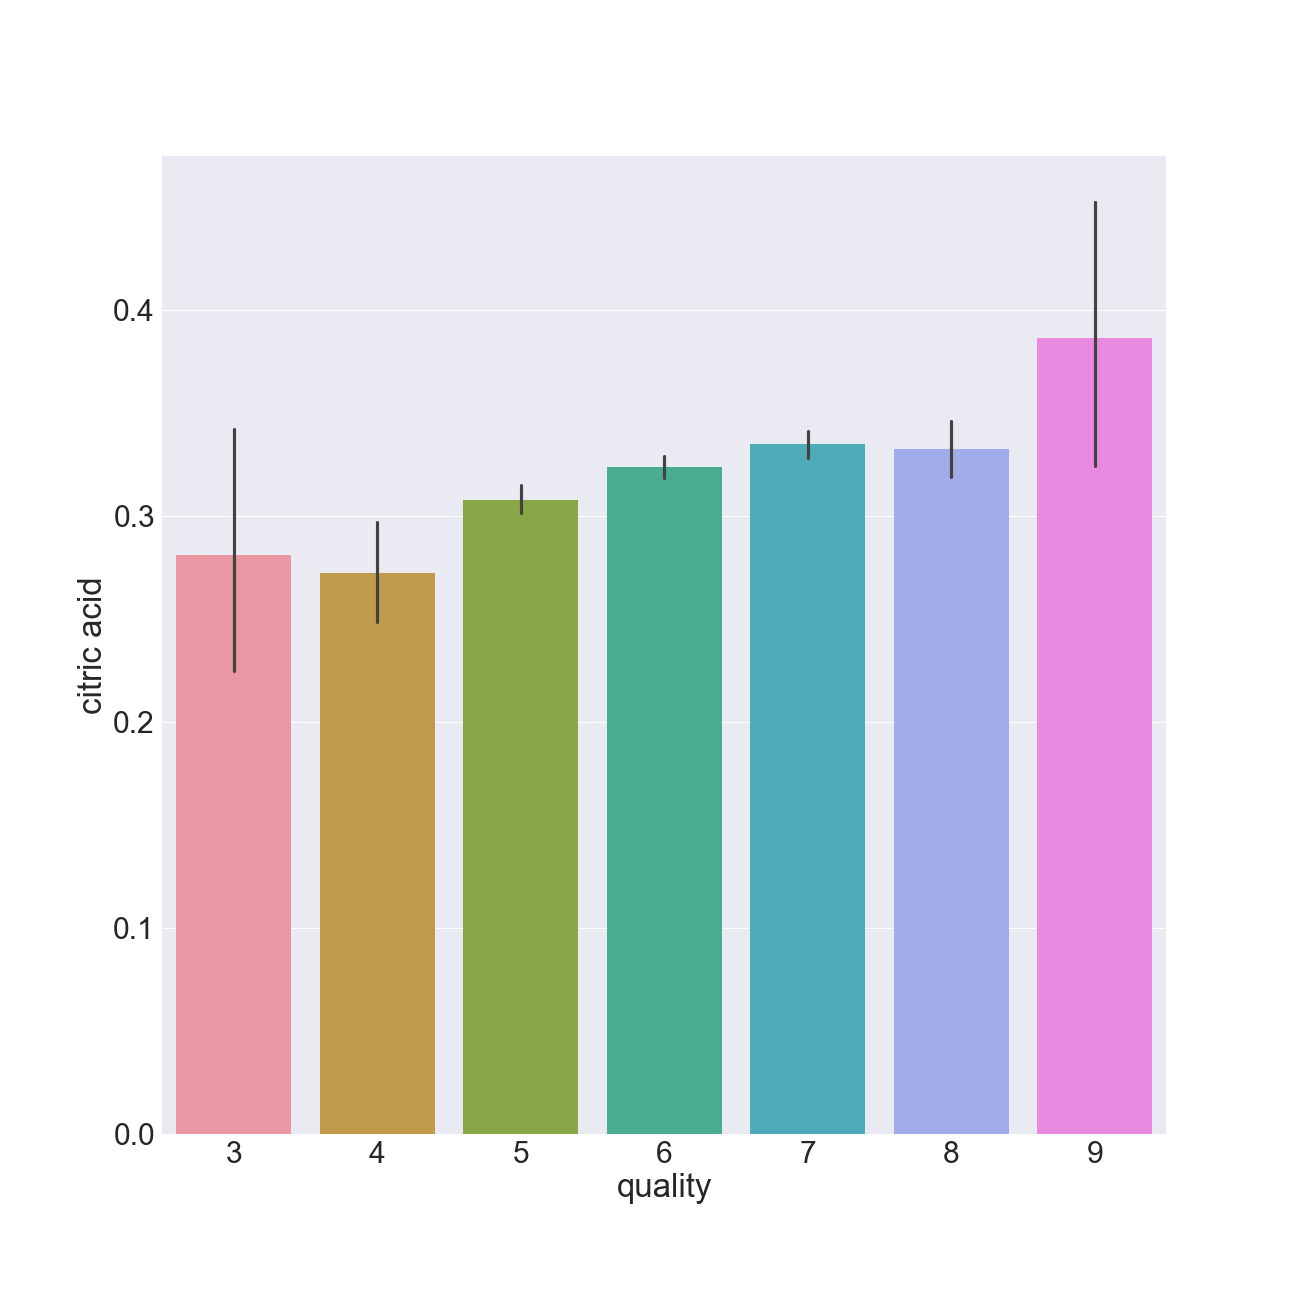
\includegraphics[width=0.5\textwidth]{Figures/citric_acid_plot.png} &
%     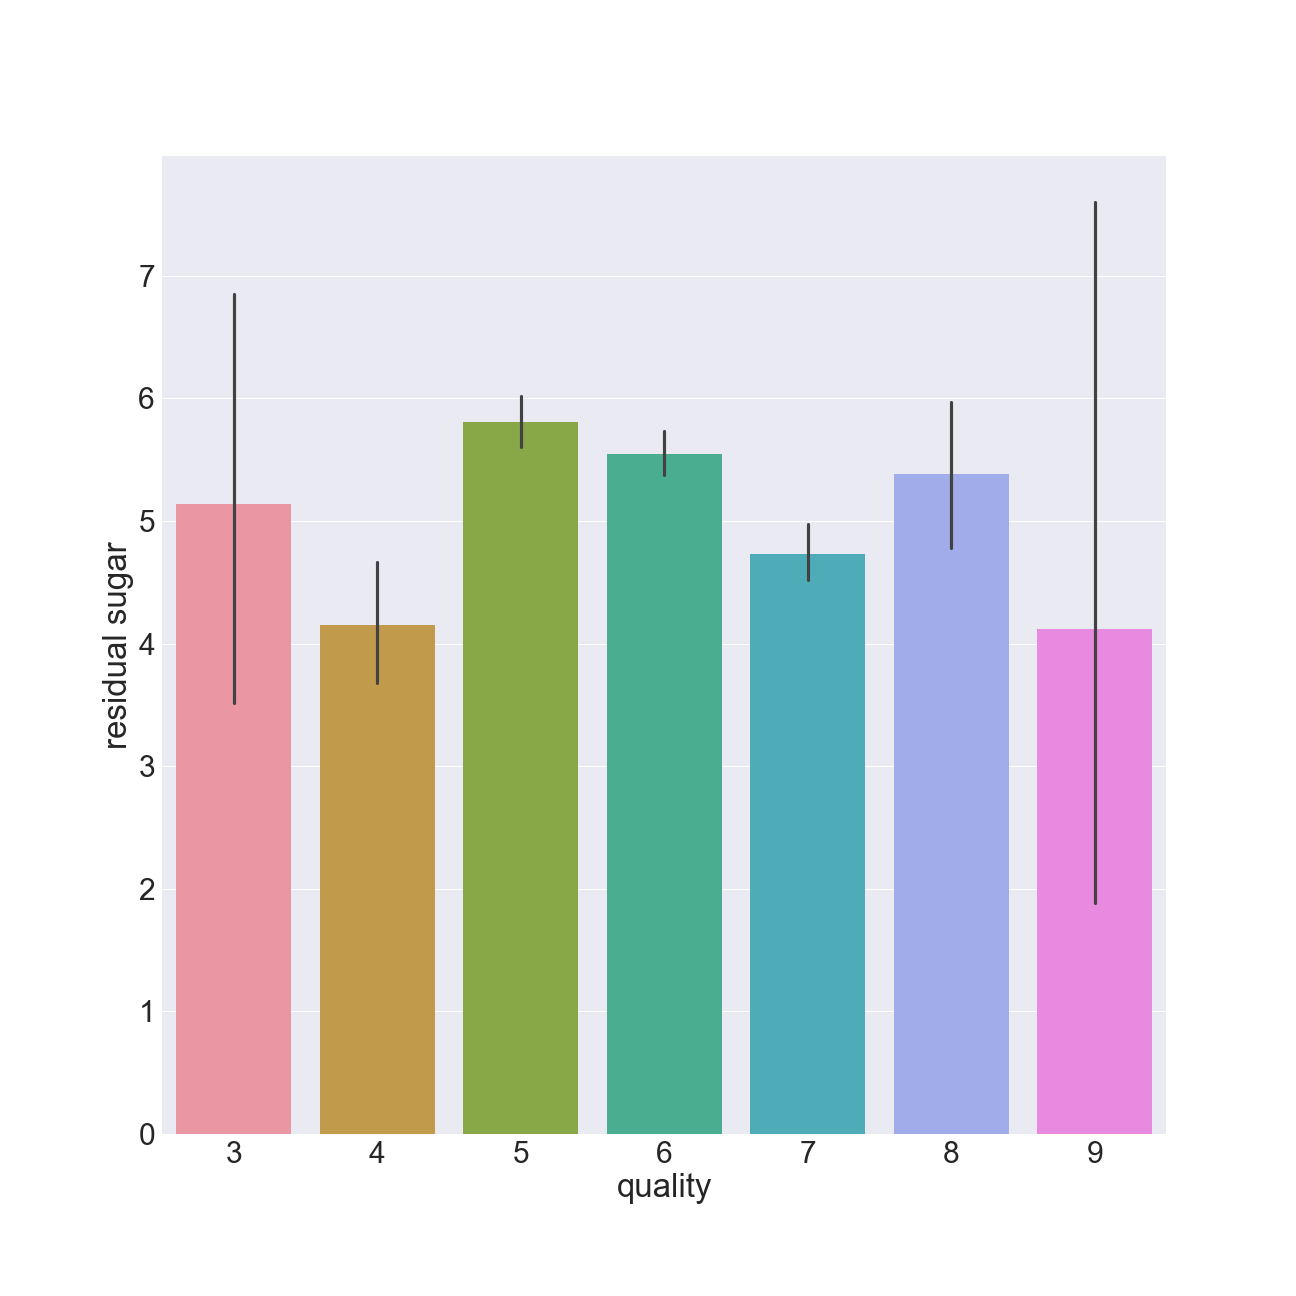
\includegraphics[width=0.5\textwidth]{Figures/residual_sugar_plot.png} \\
%     (c)  & (d)  \\[6pt]
%     \end{tabular}
    
%     \begin{tabular}{cccc}
%     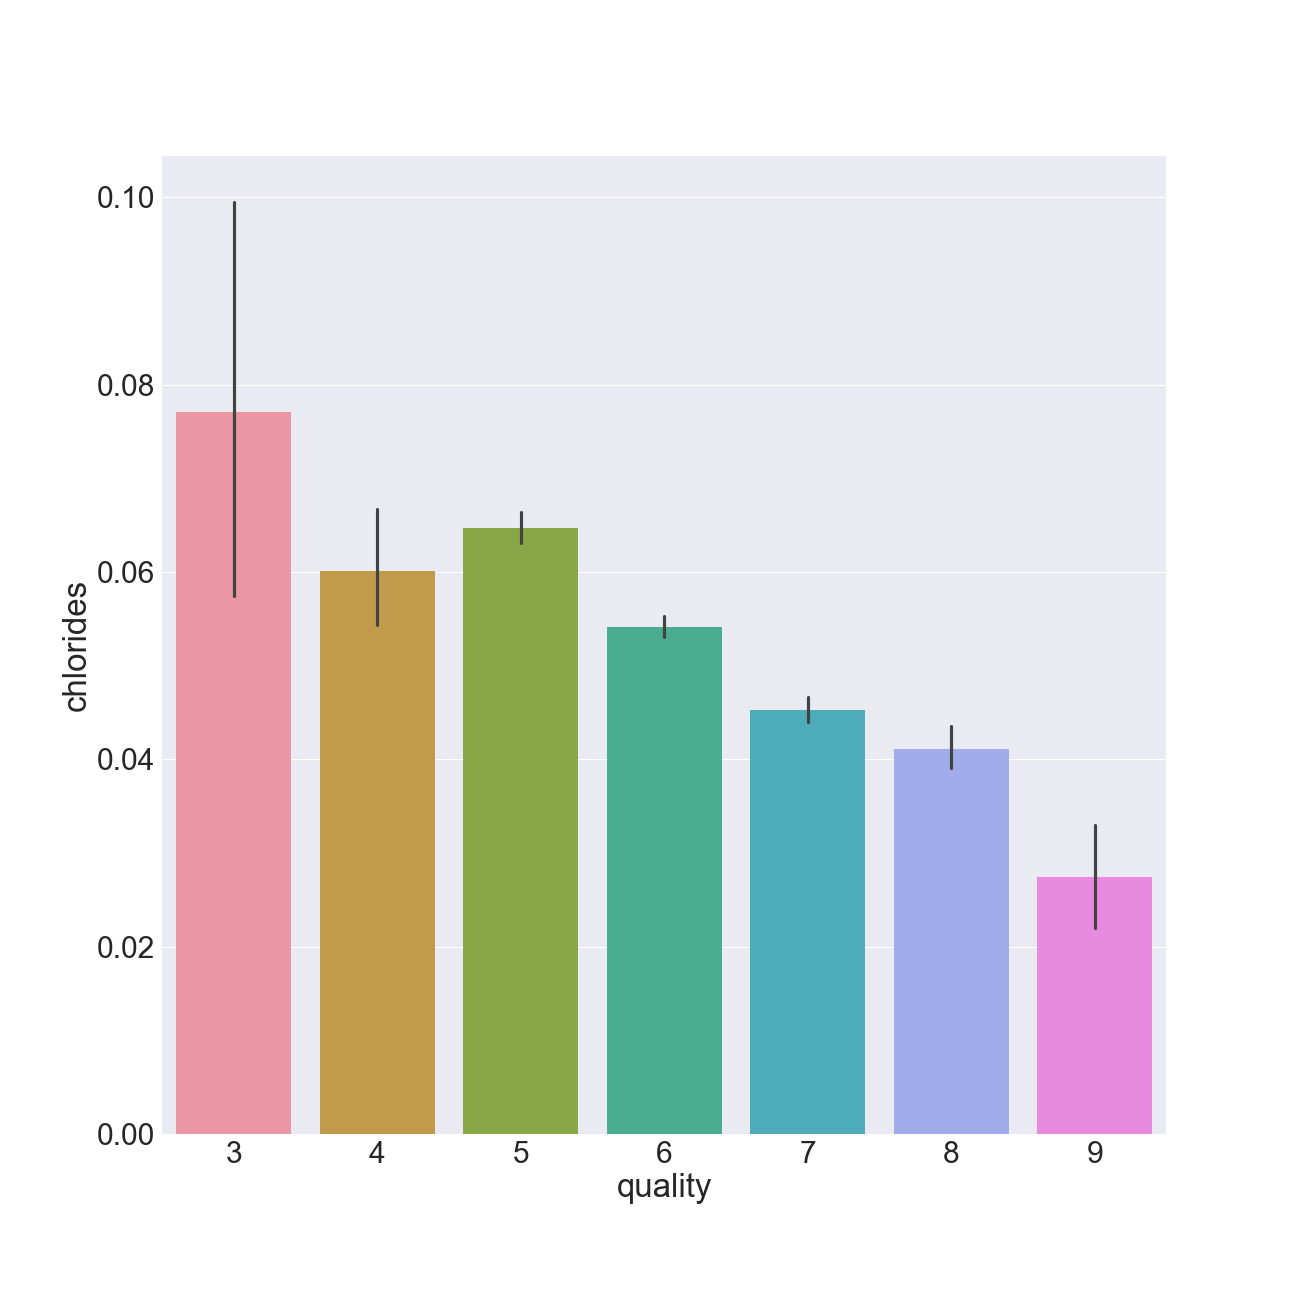
\includegraphics[width=0.5\textwidth]{Figures/chlorides_plot.png} &
%     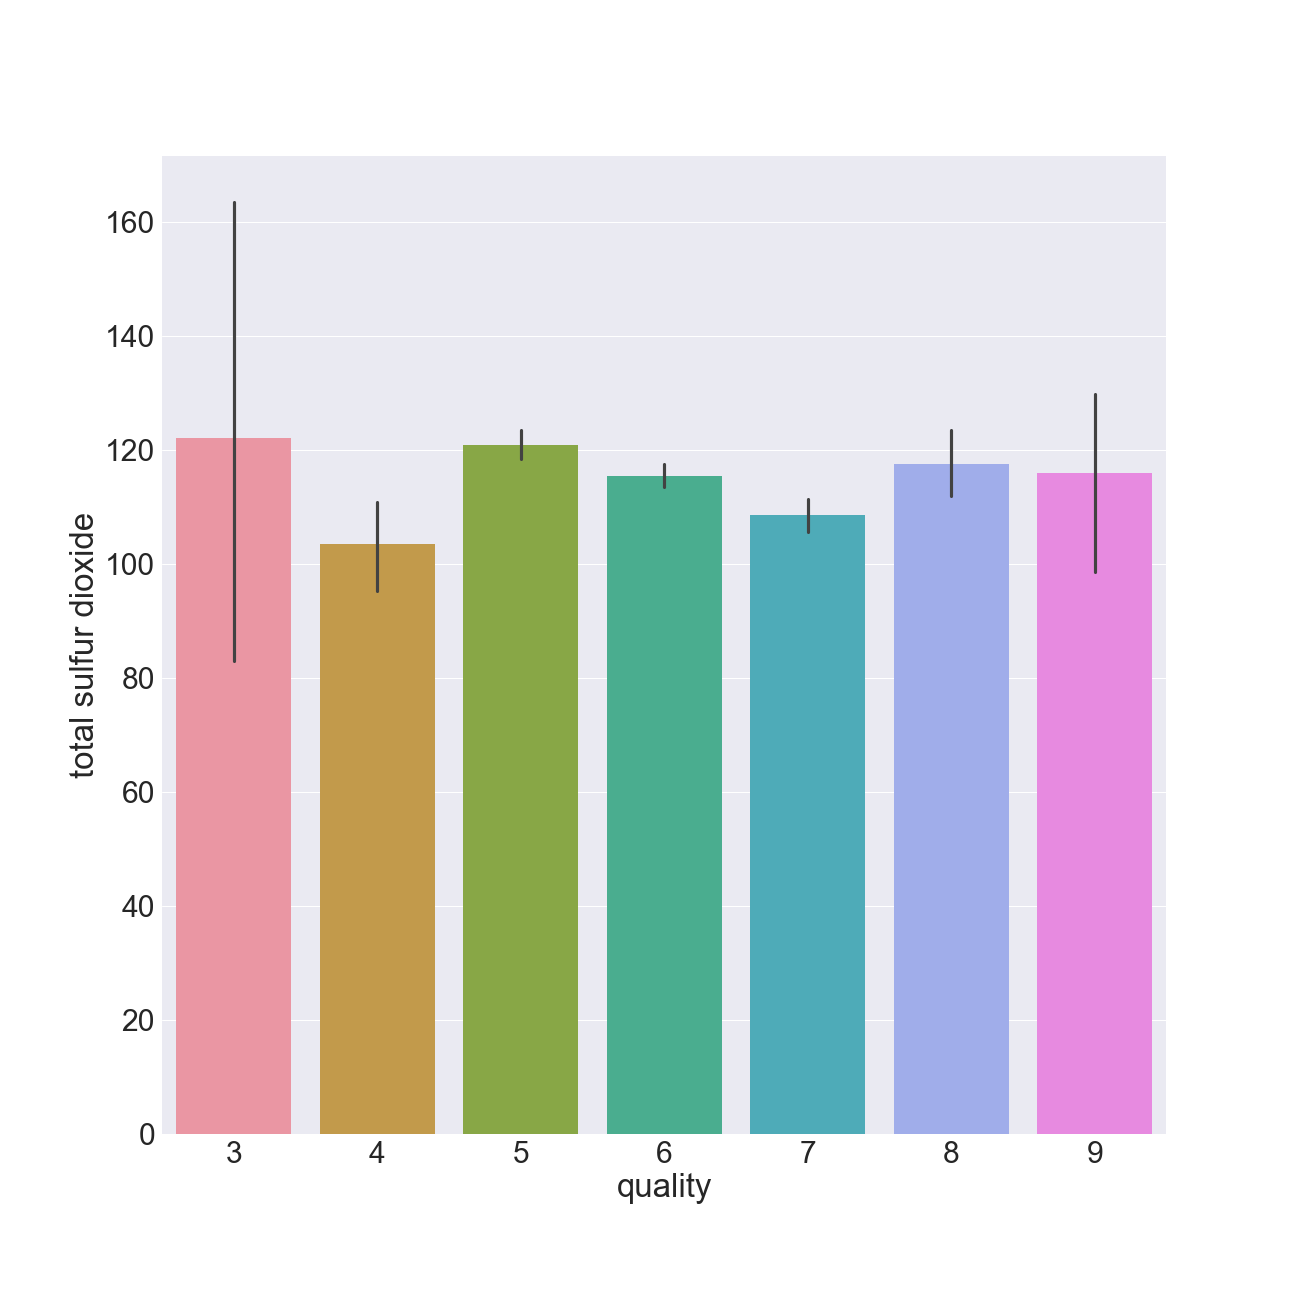
\includegraphics[width=0.5\textwidth]{Figures/total_sulfure_dioxide_plot.png} \\
%     (e)  & (f)  \\[6pt]
%     \end{tabular}
% \label{fig:wine_quality_1}
% \end{figure}
    
% \begin{figure}[H]\ContinuedFloat
%     \begin{tabular}{cccc}
%     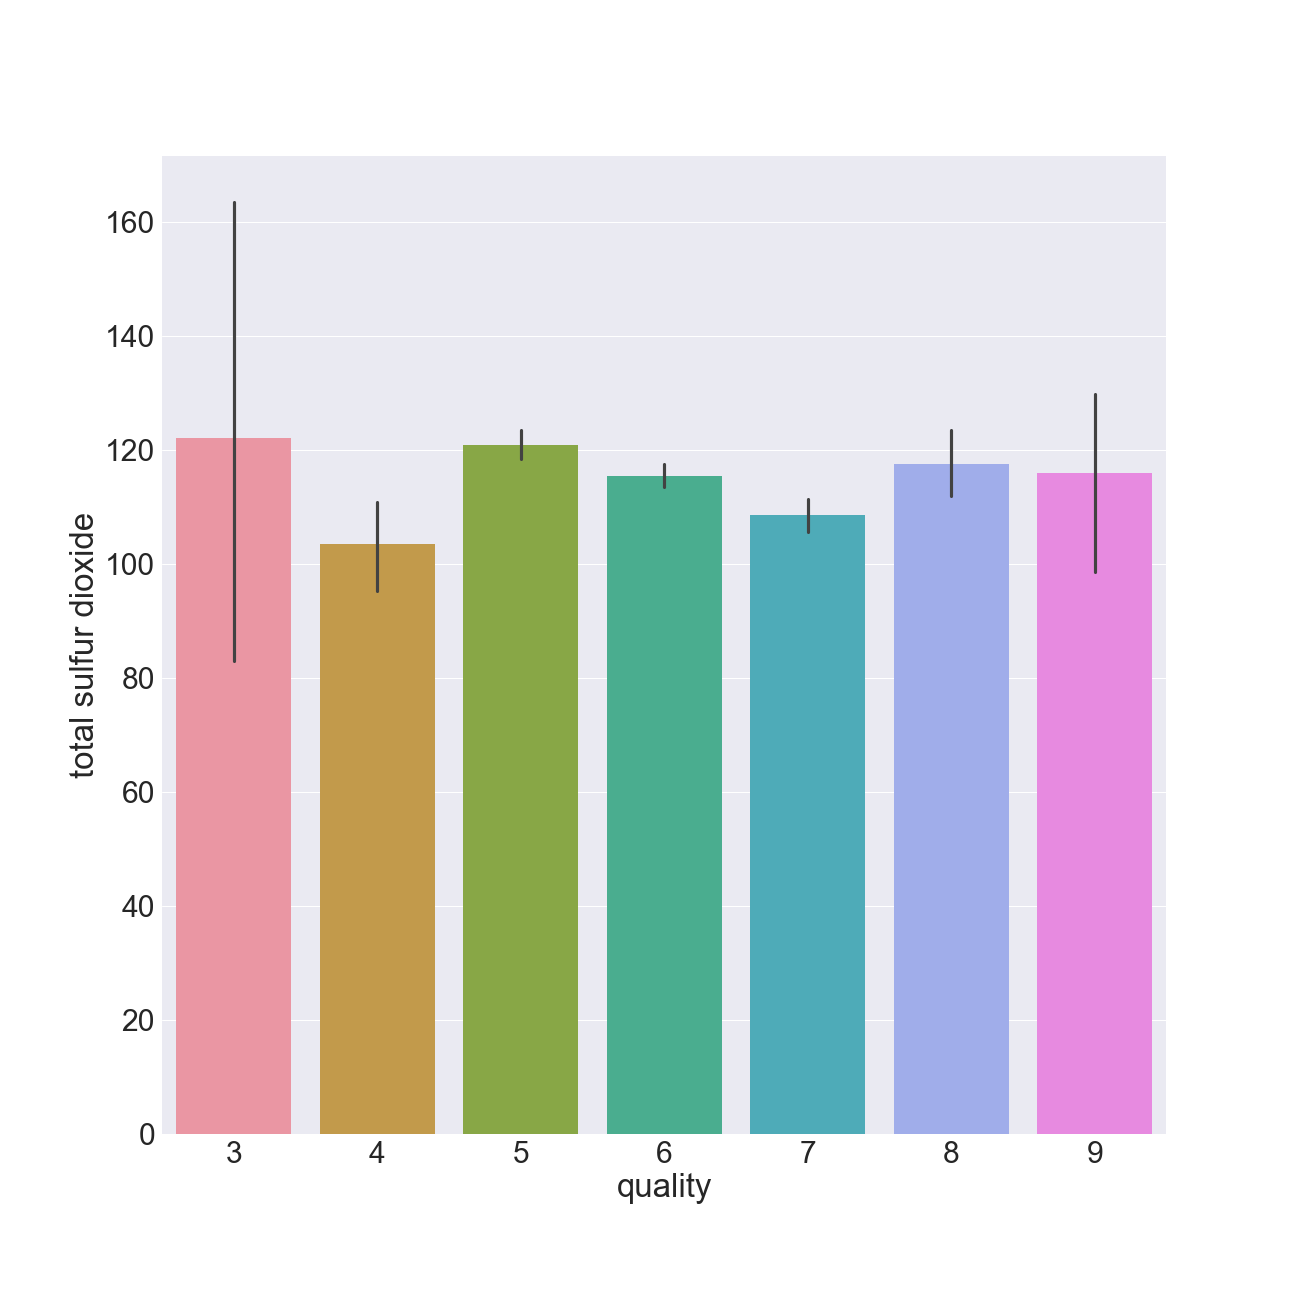
\includegraphics[width=0.5\textwidth]{Figures/total_sulfure_dioxide_plot.png} &
%     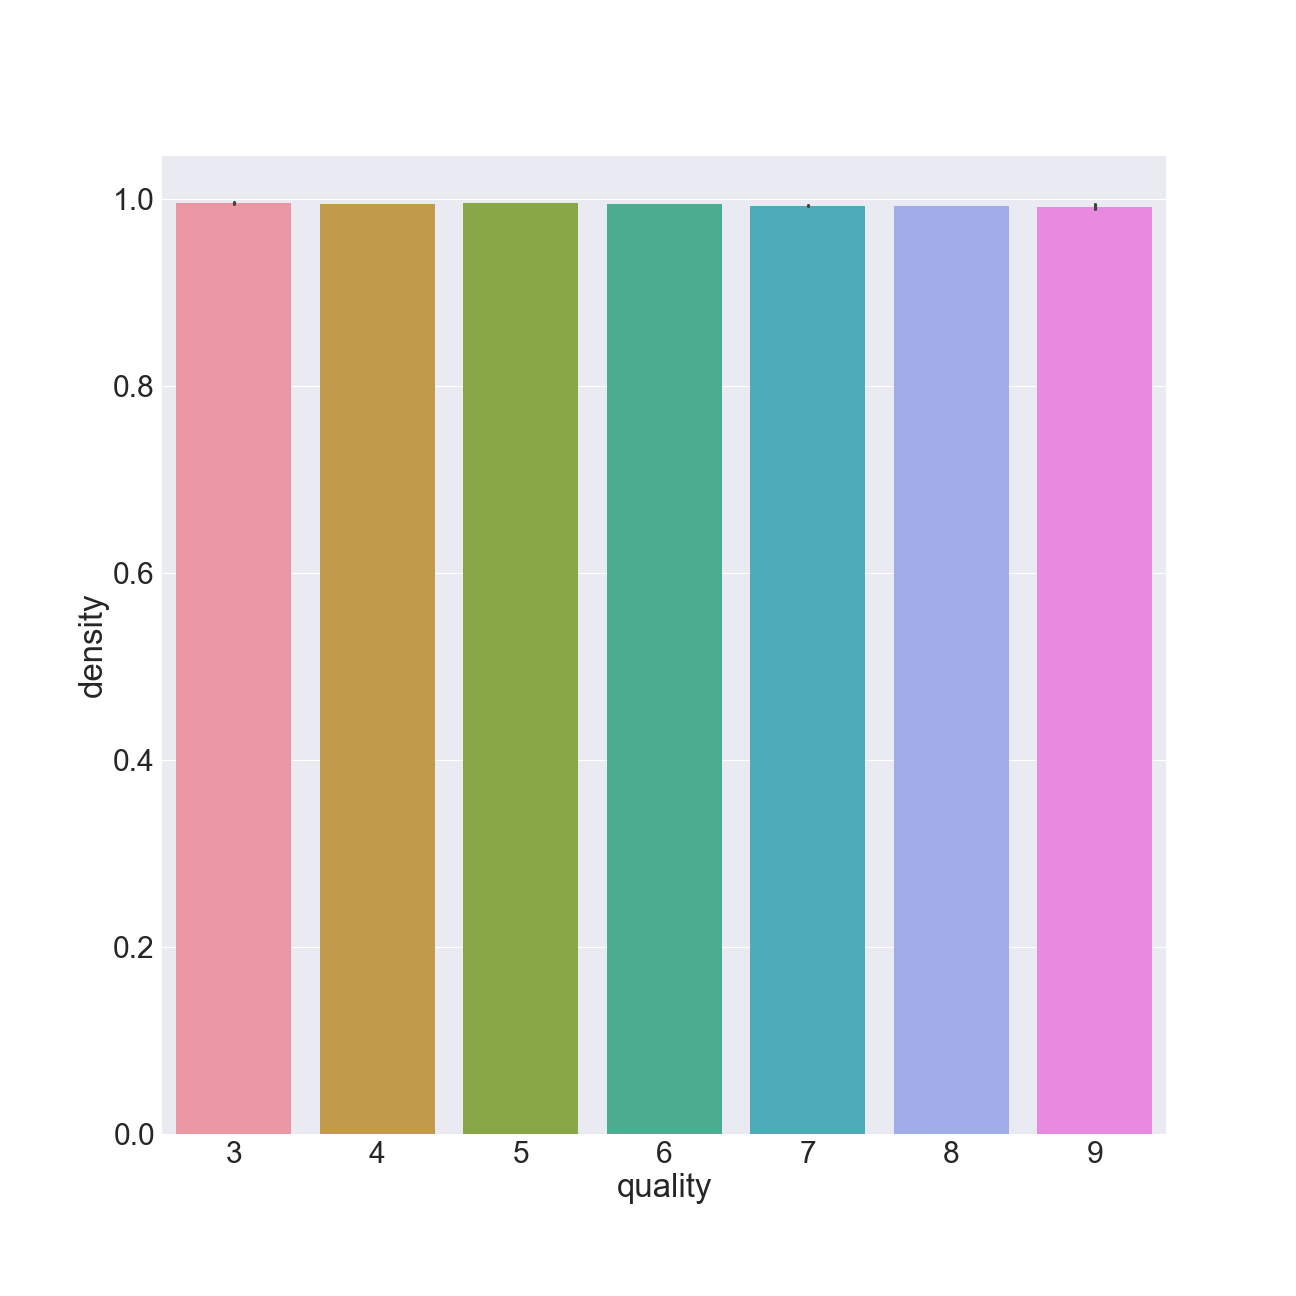
\includegraphics[width=0.5\textwidth]{Figures/density_plot.png} \\
%     (g)  & (h)  \\[6pt]
%     \end{tabular}

%     \begin{tabular}{cccc}
%     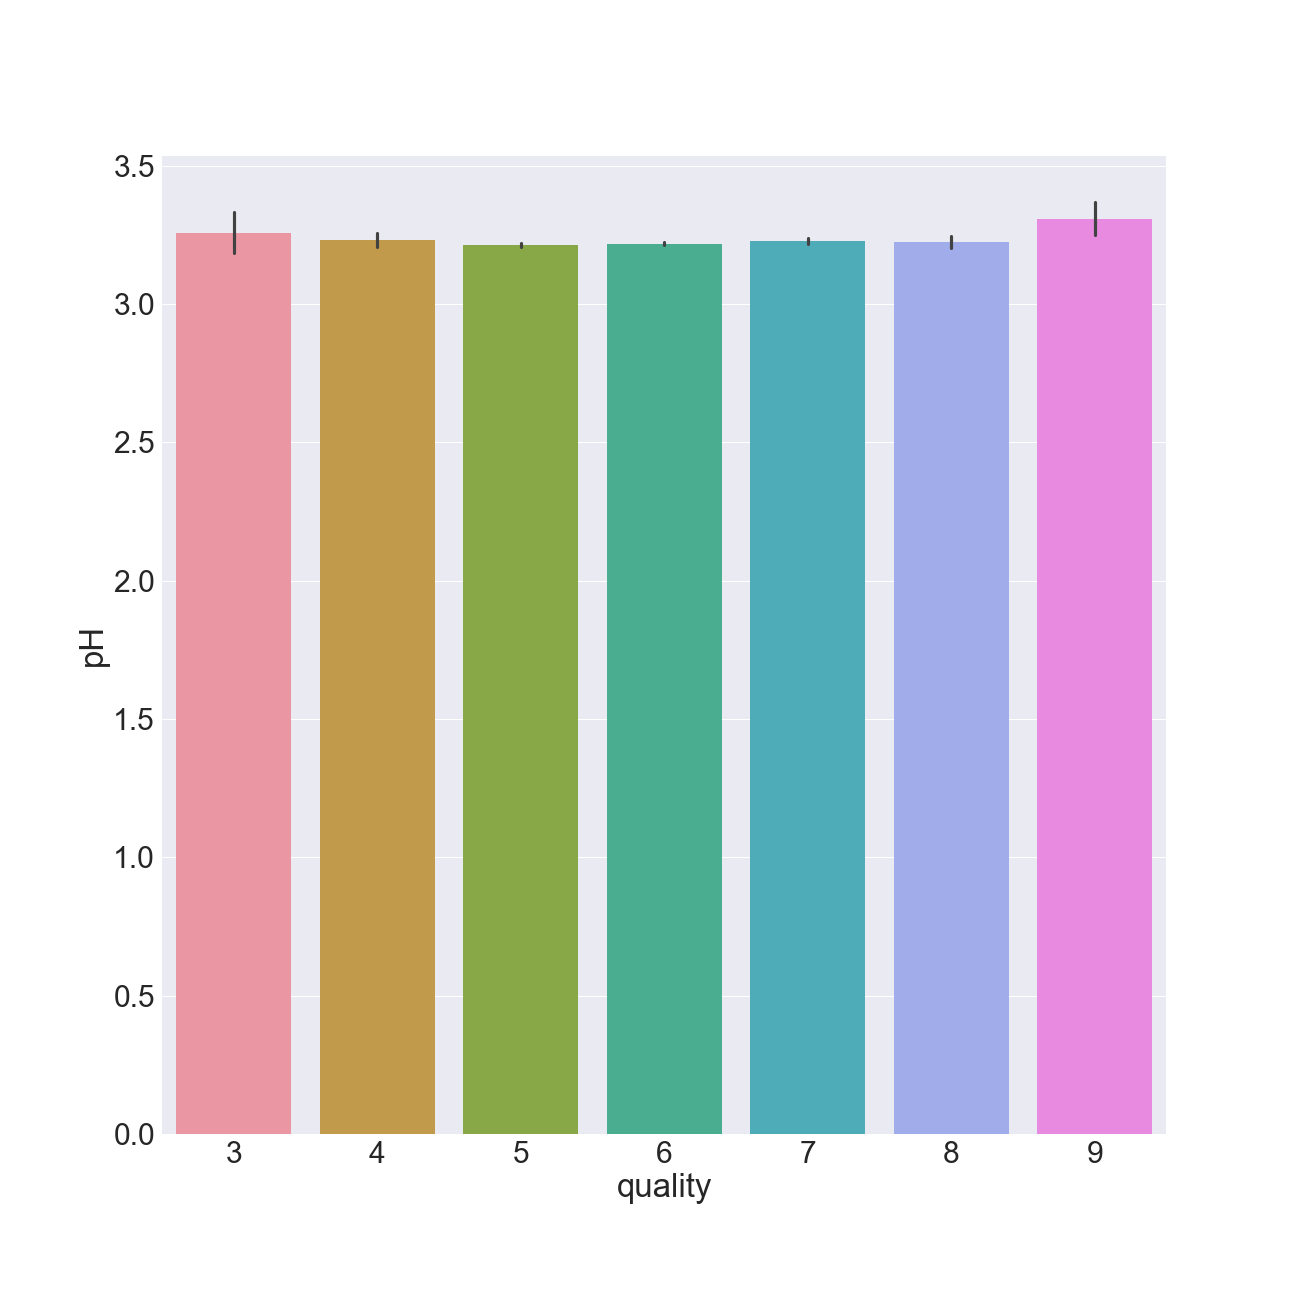
\includegraphics[width=0.5\textwidth]{Figures/pH_plot.png} &
%     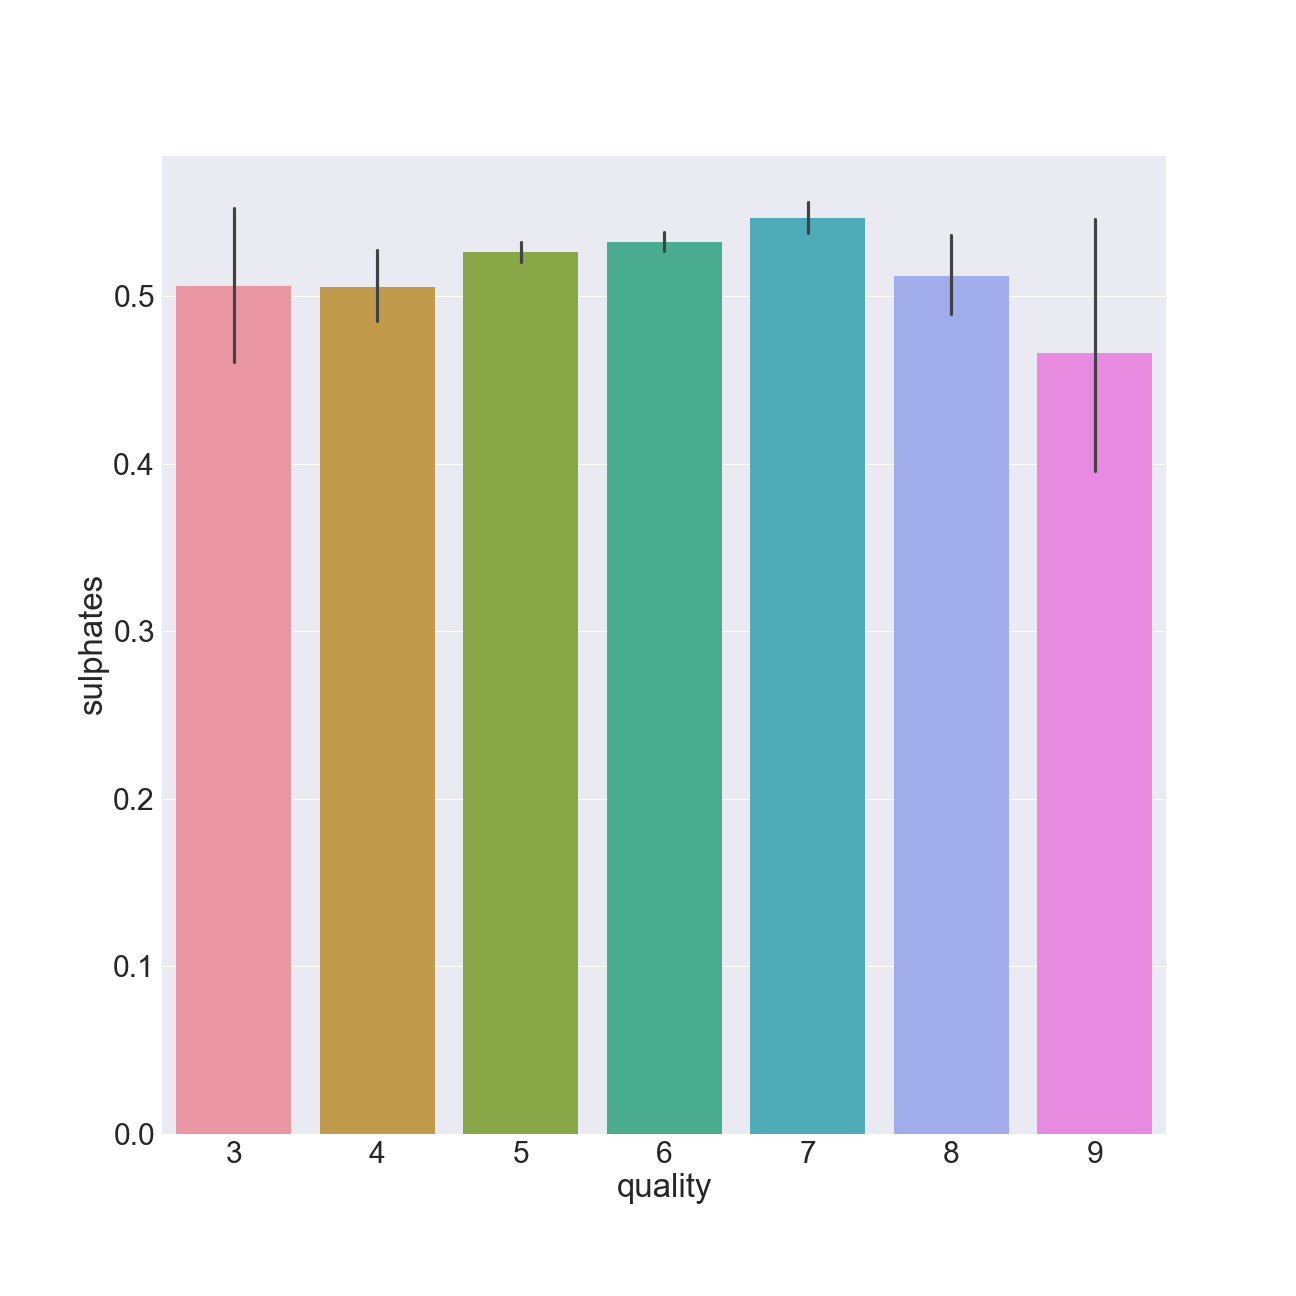
\includegraphics[width=0.5\textwidth]{Figures/sulphates_plot.png} \\
%     (i)  & (j)  \\[6pt]
%     \end{tabular}
    
%     \begin{tabular}{cccc}
%     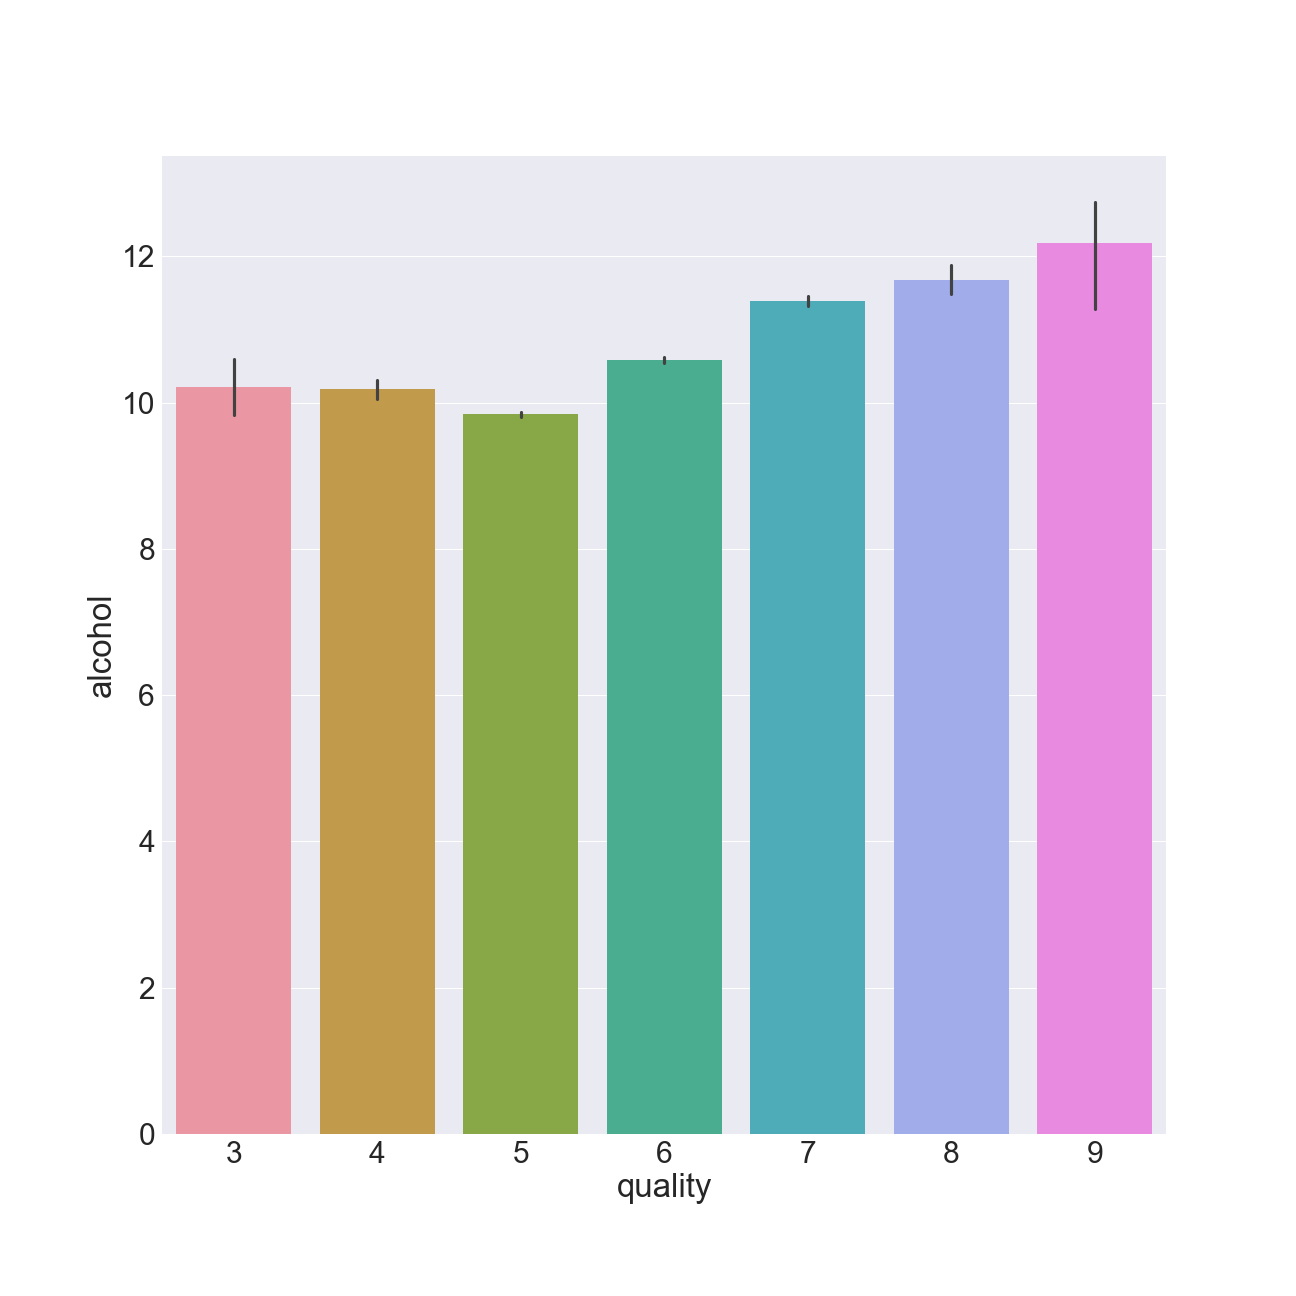
\includegraphics[width=0.5\textwidth]{Figures/alcohol_plot.png} \\
%     (k)  \\[6pt]
%     \end{tabular}
% \caption{Wine quality with respect to (a) fixed acidity, (b) volatile acidity, (c) citric acid, (d) residual sugar, (e) chlorides, (f) total sulfur dioxide, (g) total sulfur dioxide, (h) density, (i) pH, (j) sulphate and (k) alcohol}
% \label{fig:wine_quality_2}
% \end{figure}

% \begin{figure} [H]
%     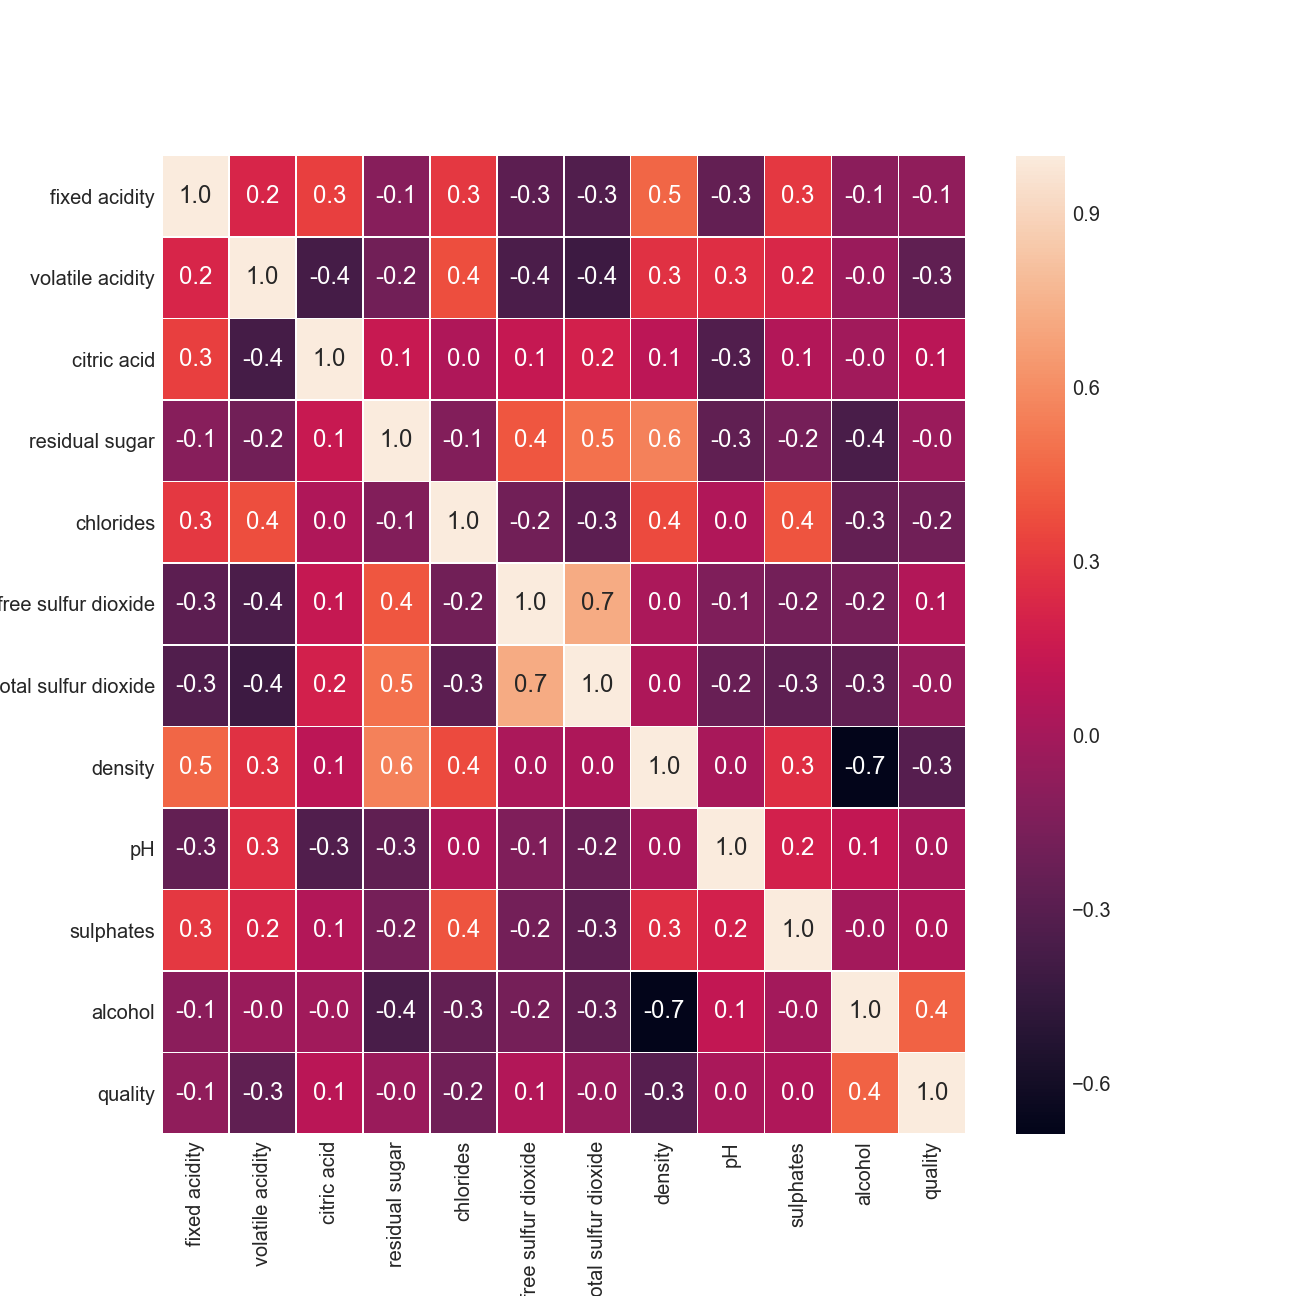
\includegraphics[width=1\textwidth]{Figures/heatmap_plot.png}
% \caption{Correlation matrix}
% \label{distribution_wine}
% \end{figure}

\begin{figure} [H]
    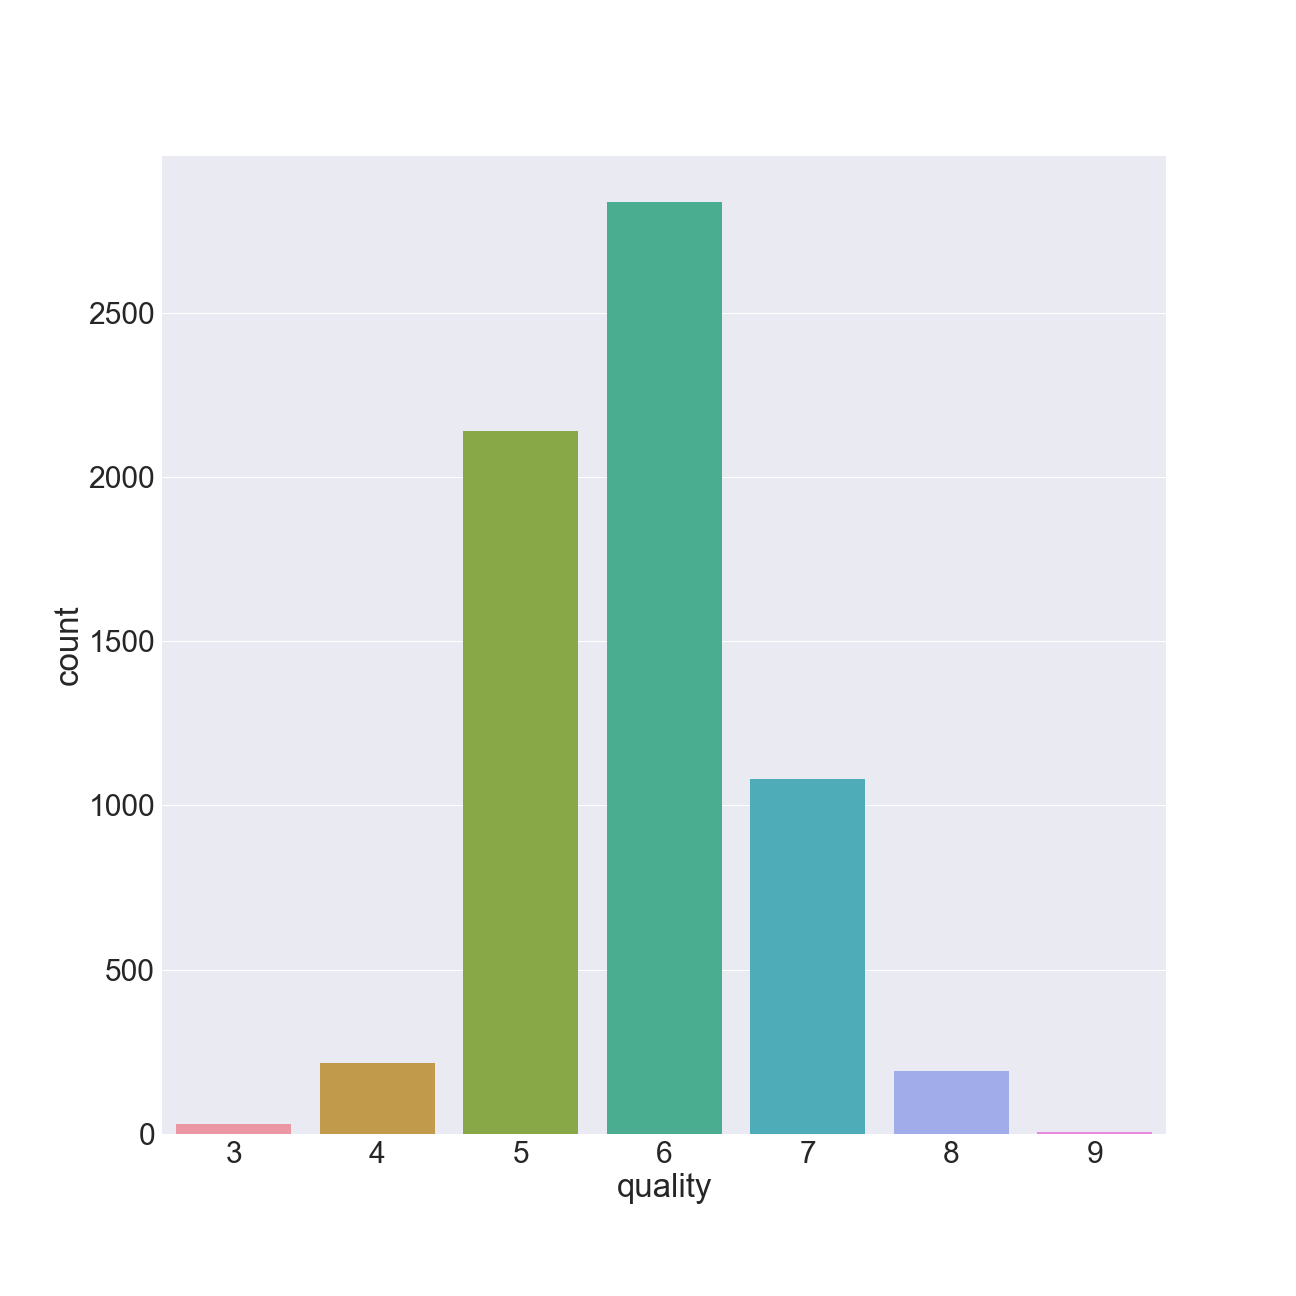
\includegraphics[width=1\textwidth]{Figures/instances.png}
\caption{Distribution of the data}
\end{figure}

\section{Forest Cover Type dataset analysis}
\label{Annexe_ForestAnalysis}

% \begin{figure} [H]
% \centering
%     \begin{tabular}{cccc}
%     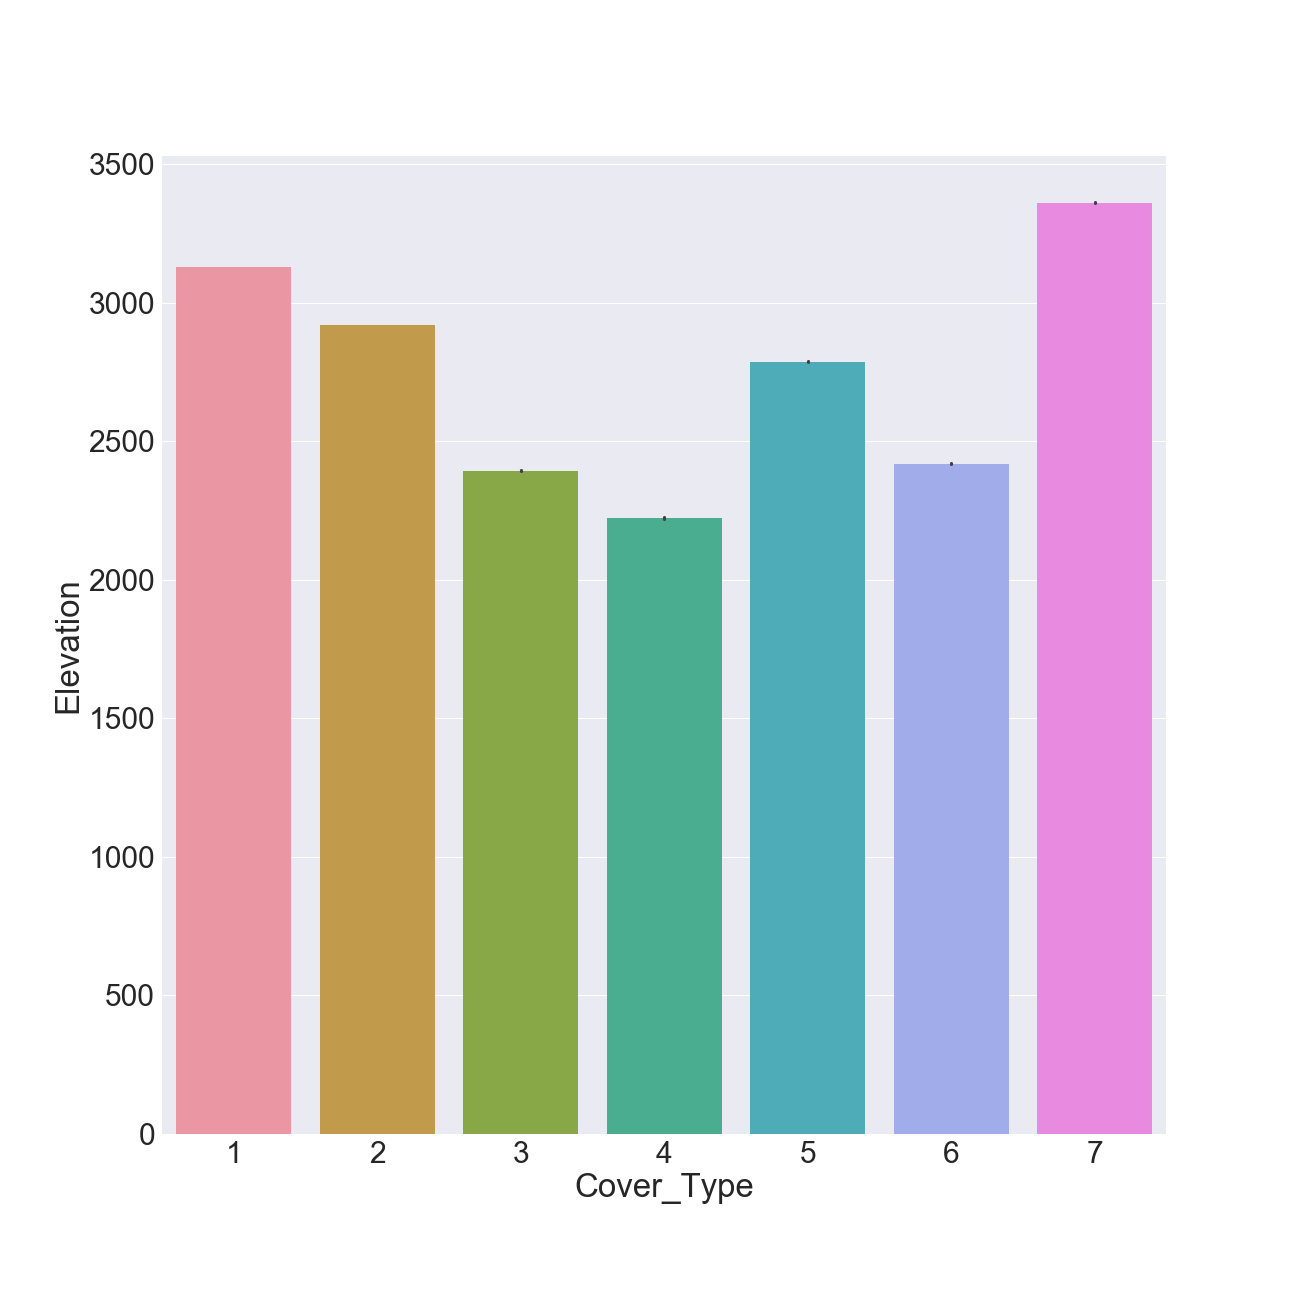
\includegraphics[width=0.5\textwidth]{Figures/elevation_plot_forest.png} &
%     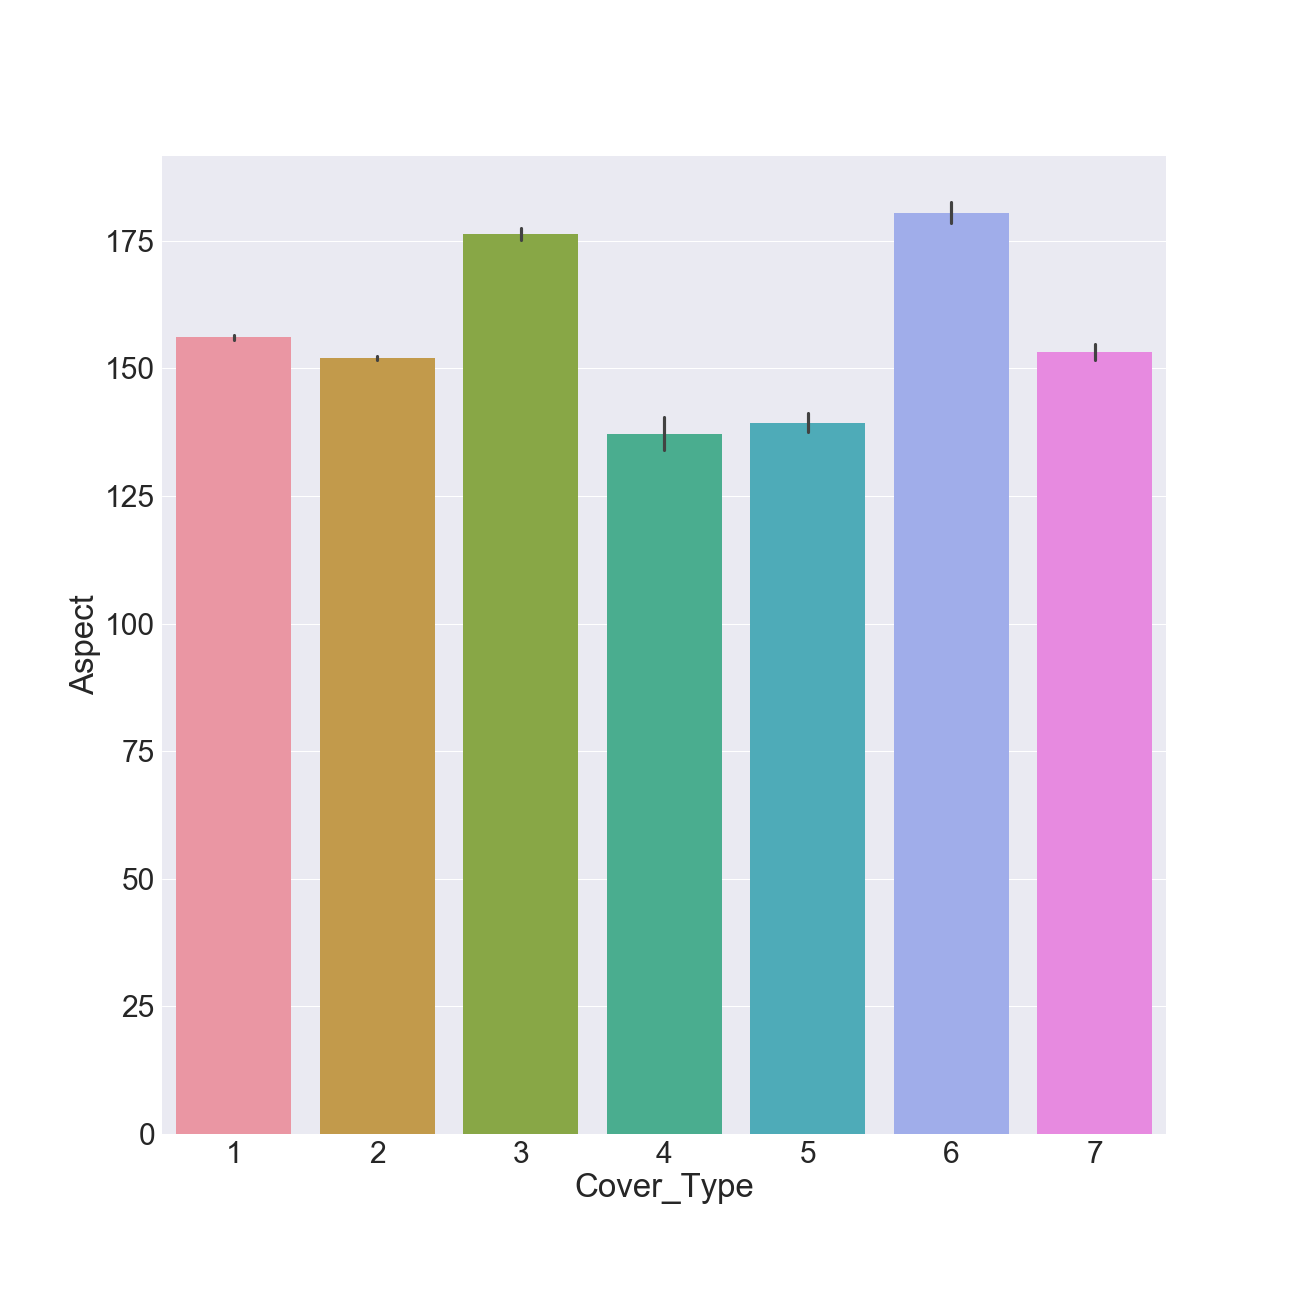
\includegraphics[width=0.5\textwidth]{Figures/Aspect_forest.png}  \\
%     (a)  & (b) \\[6pt]
%     \end{tabular}
%     \begin{tabular}{cccc}
%     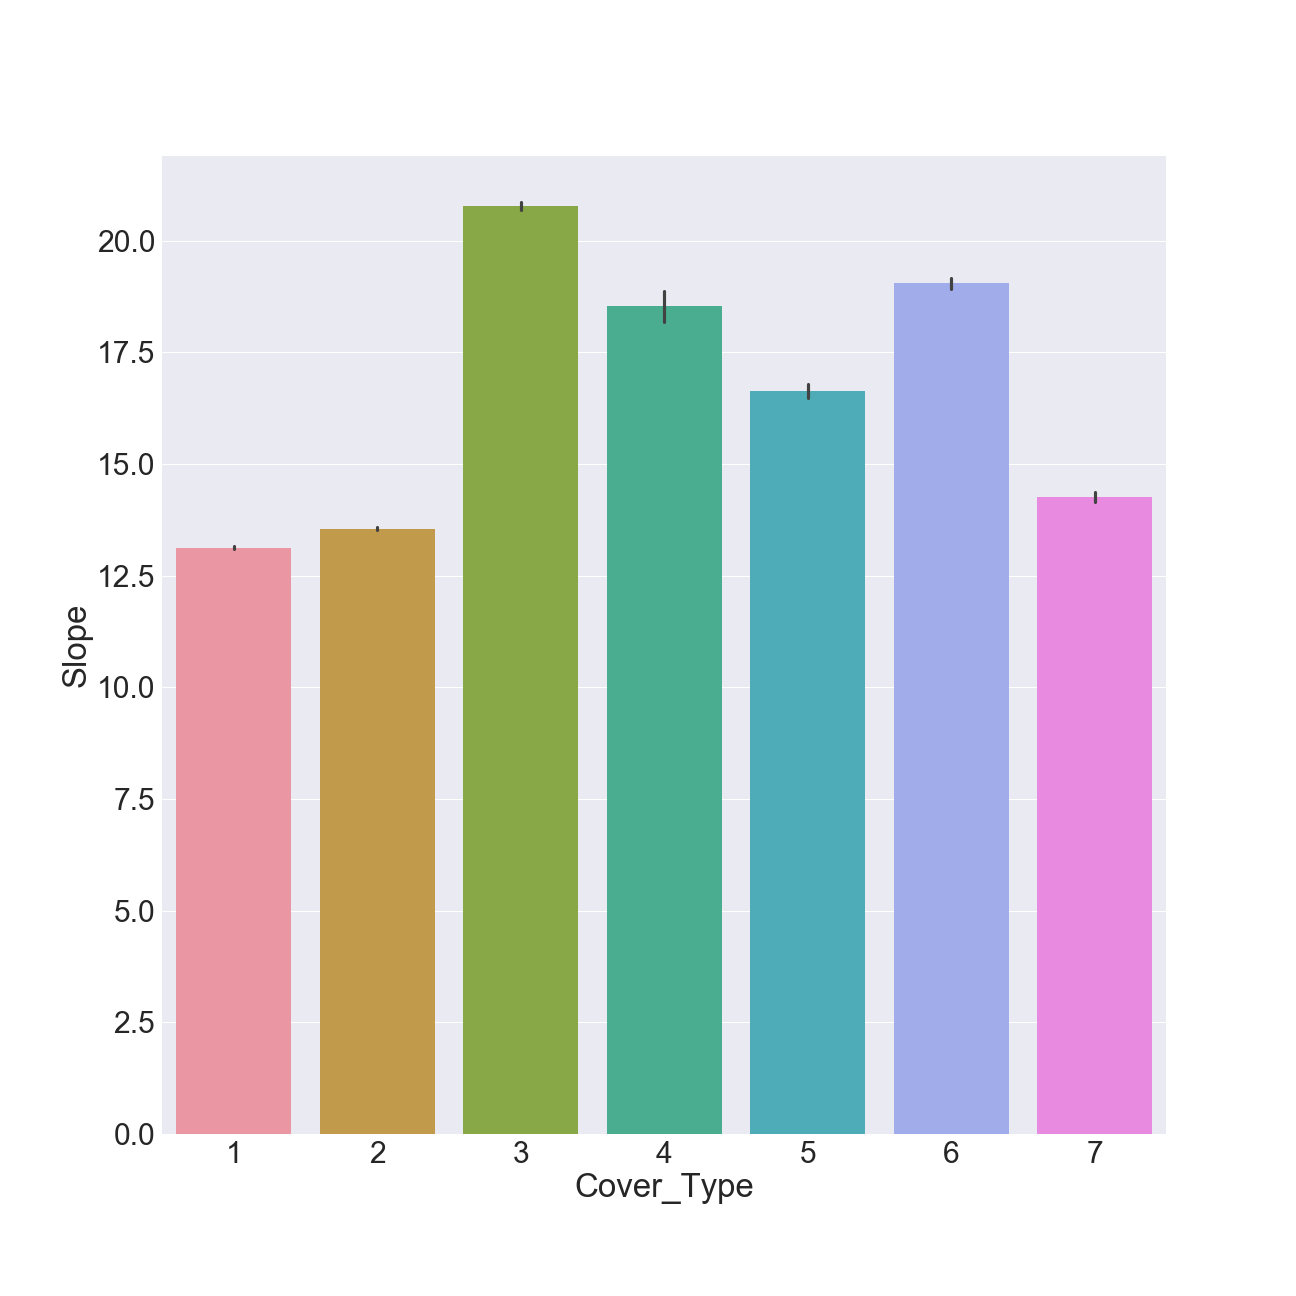
\includegraphics[width=0.5\textwidth]{Figures/Slope_forest.png} &
%     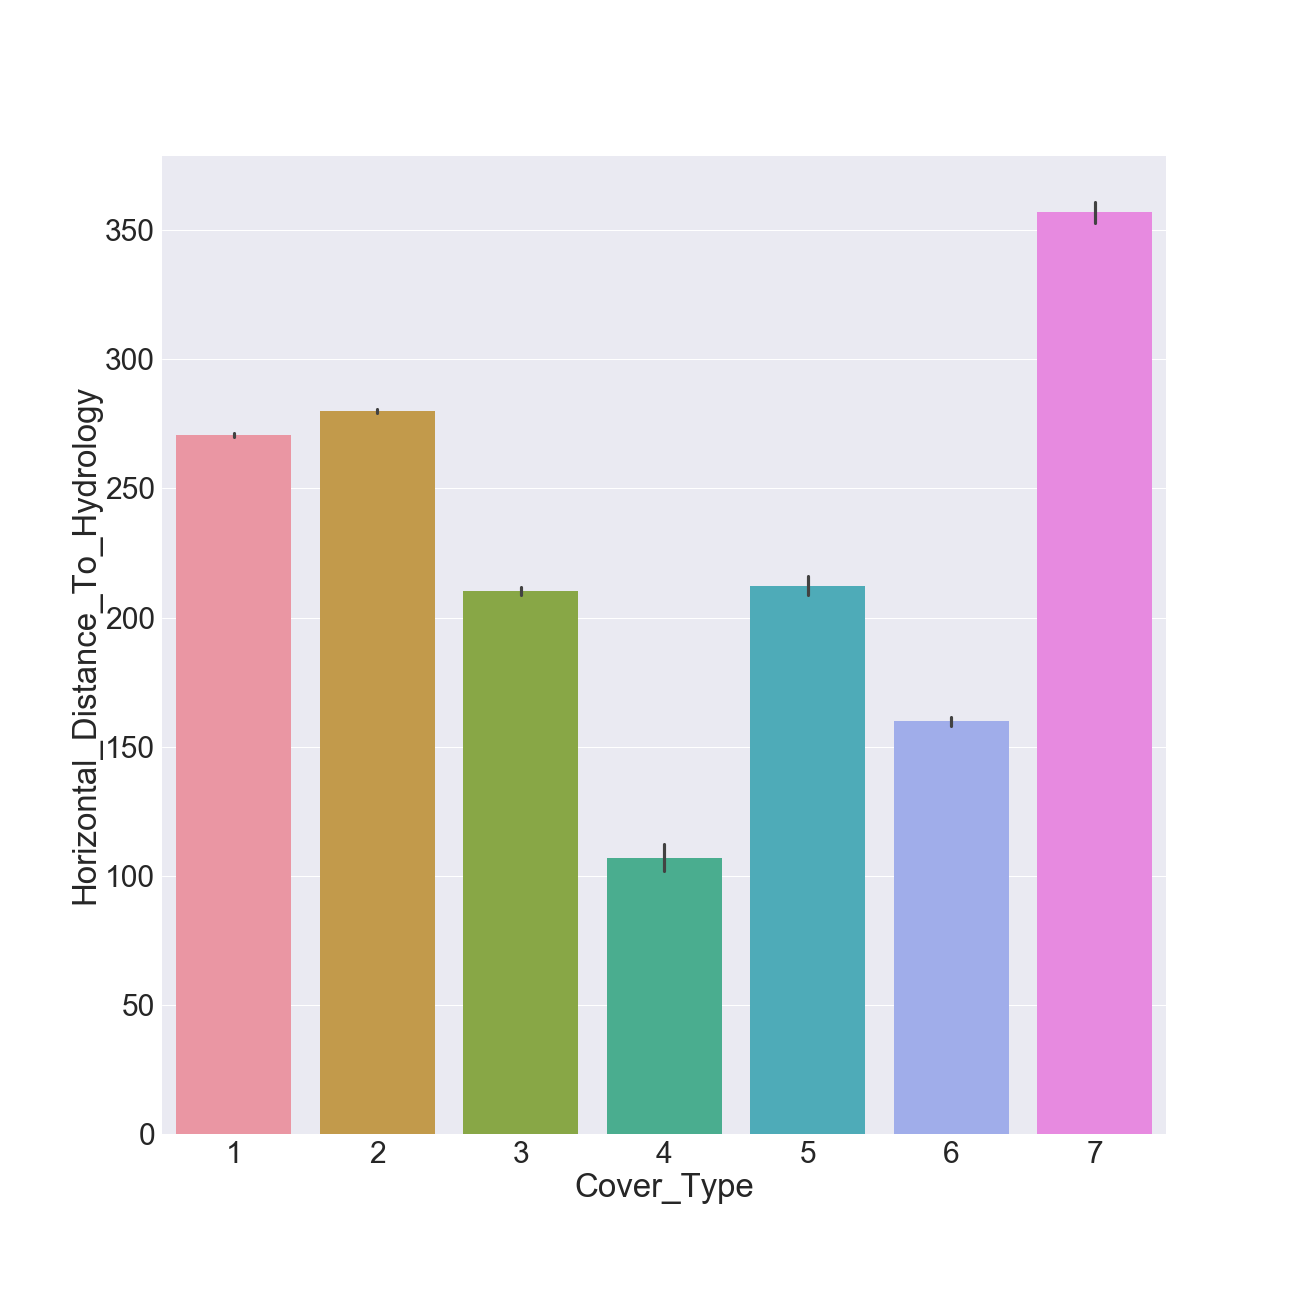
\includegraphics[width=0.5\textwidth]{Figures/Horizontal_Distance_To_Hydrology_forest.png} \\
%     (c)  & (d)  \\[6pt]
%     \end{tabular}
    
%     \begin{tabular}{cccc}
%     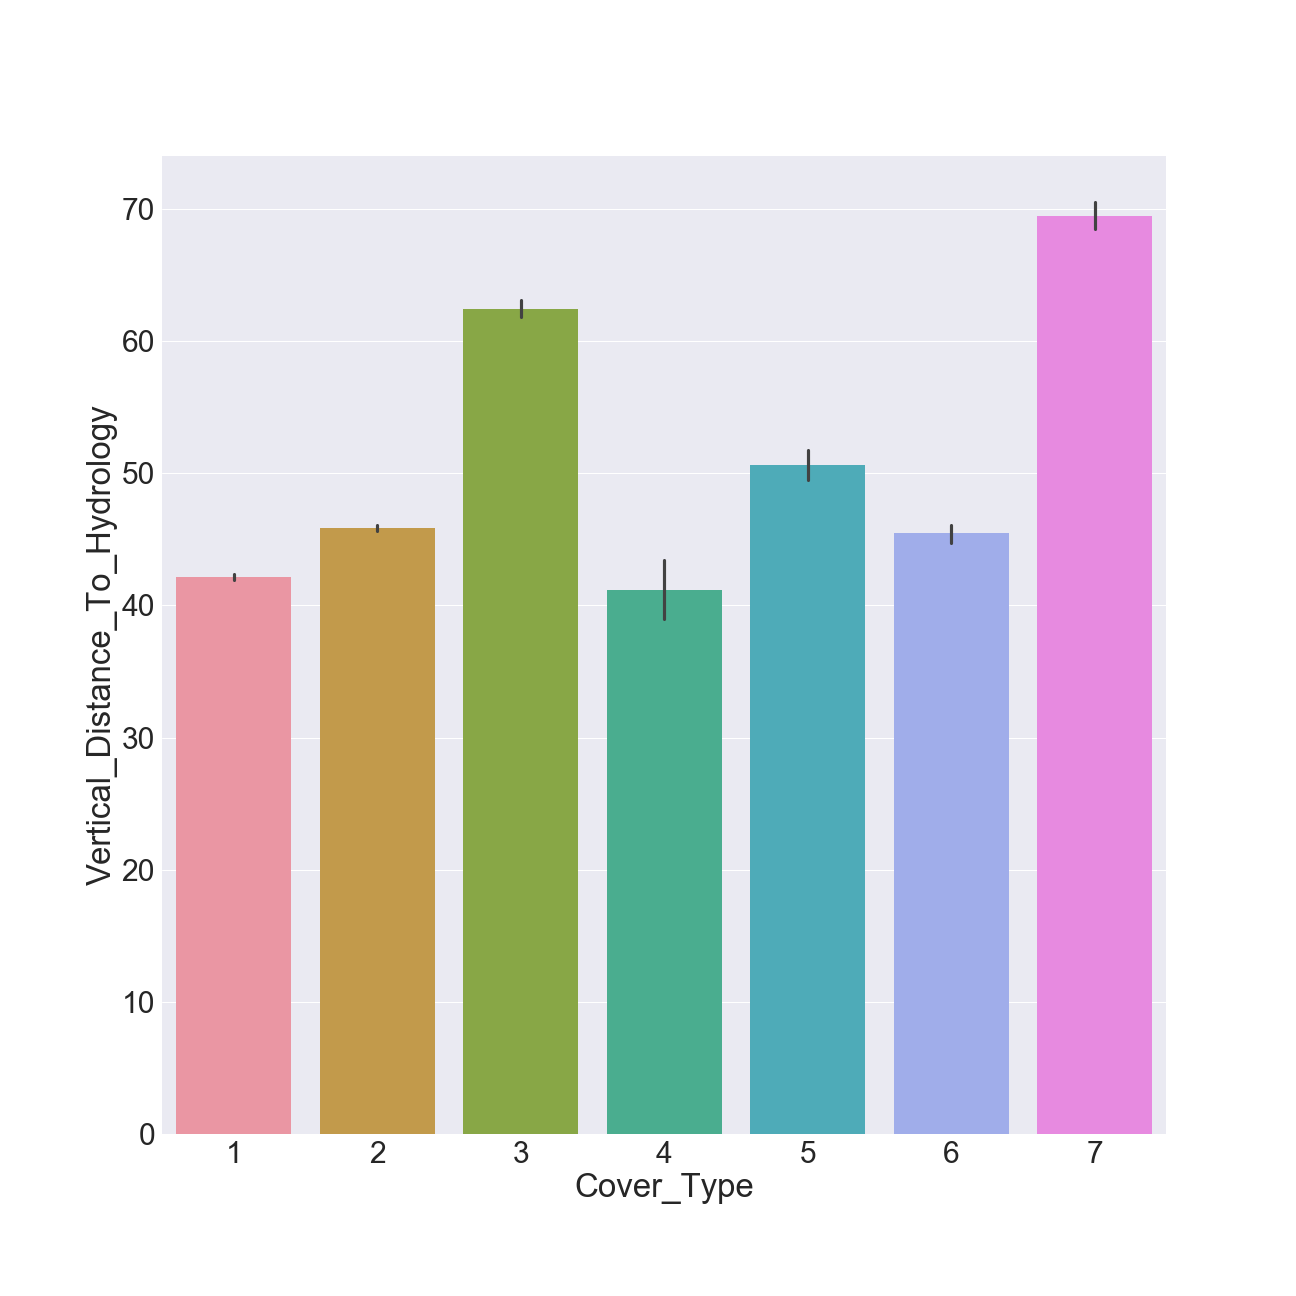
\includegraphics[width=0.5\textwidth]{Figures/Vertical_Distance_To_Hydrology_forest.png} &
%     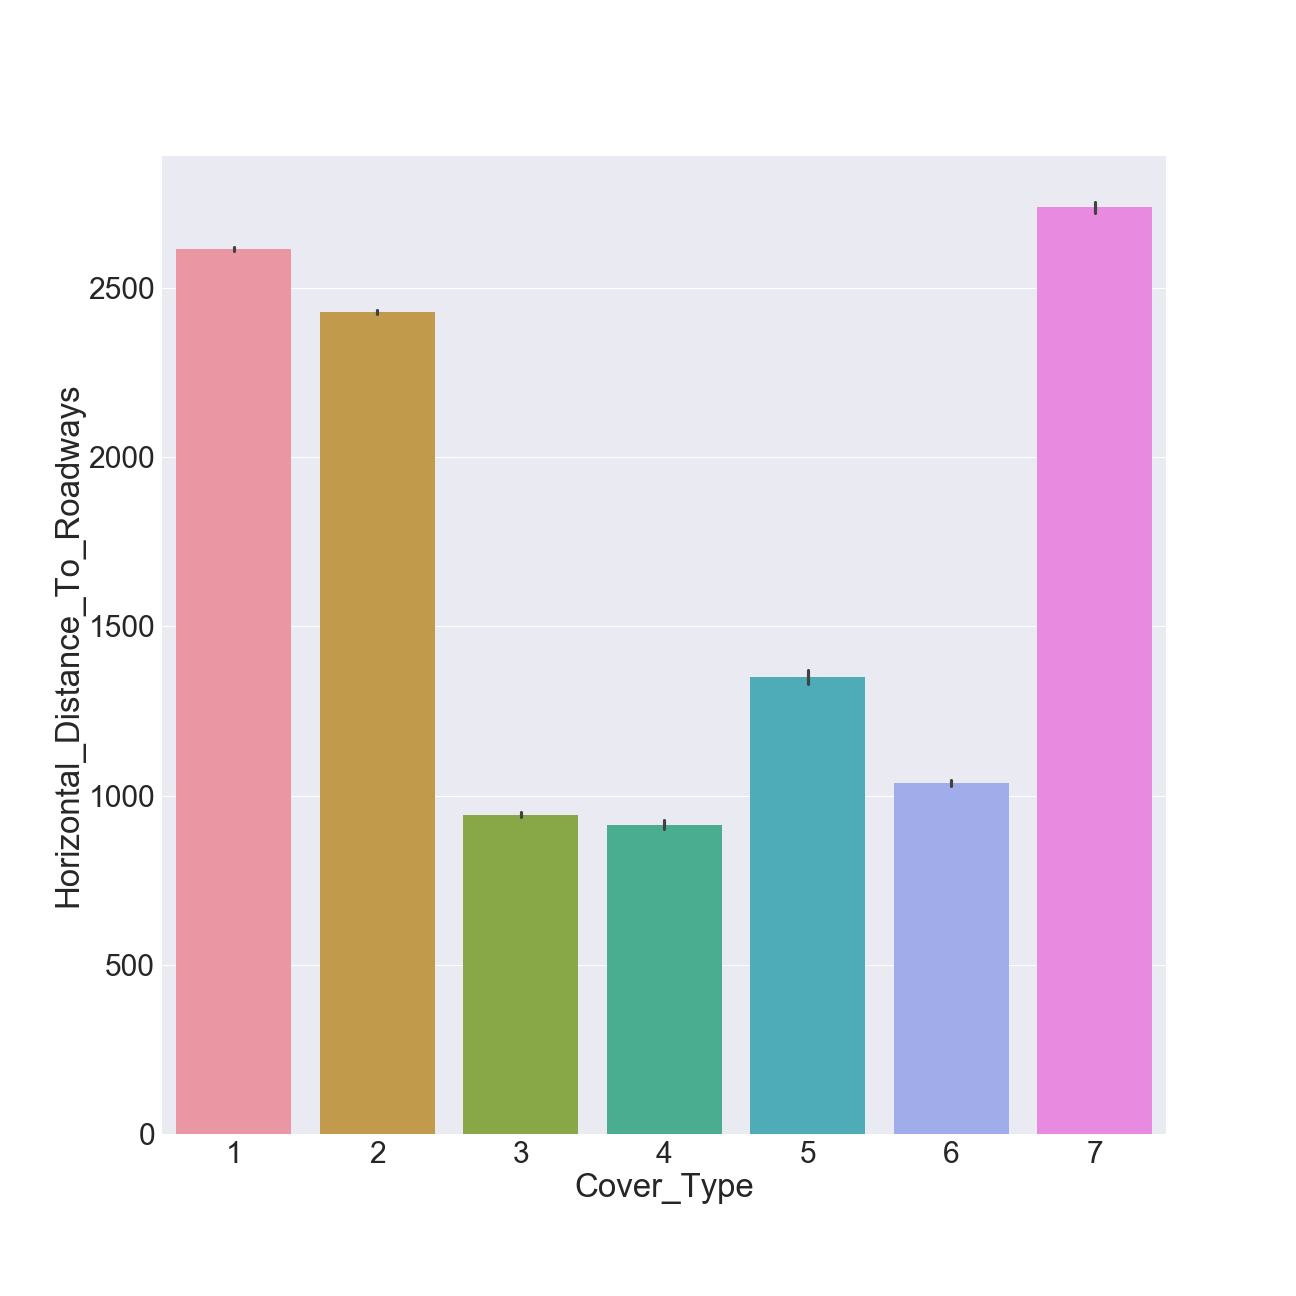
\includegraphics[width=0.5\textwidth]{Figures/Horizontal_Distance_To_Roadways_forest.png} \\
%     (e)  & (f)  \\[6pt]
%     \end{tabular}
% \label{fig:wine_quality_1}
% \end{figure}
    
% \begin{figure}[H]\ContinuedFloat
%     \begin{tabular}{cccc}
%     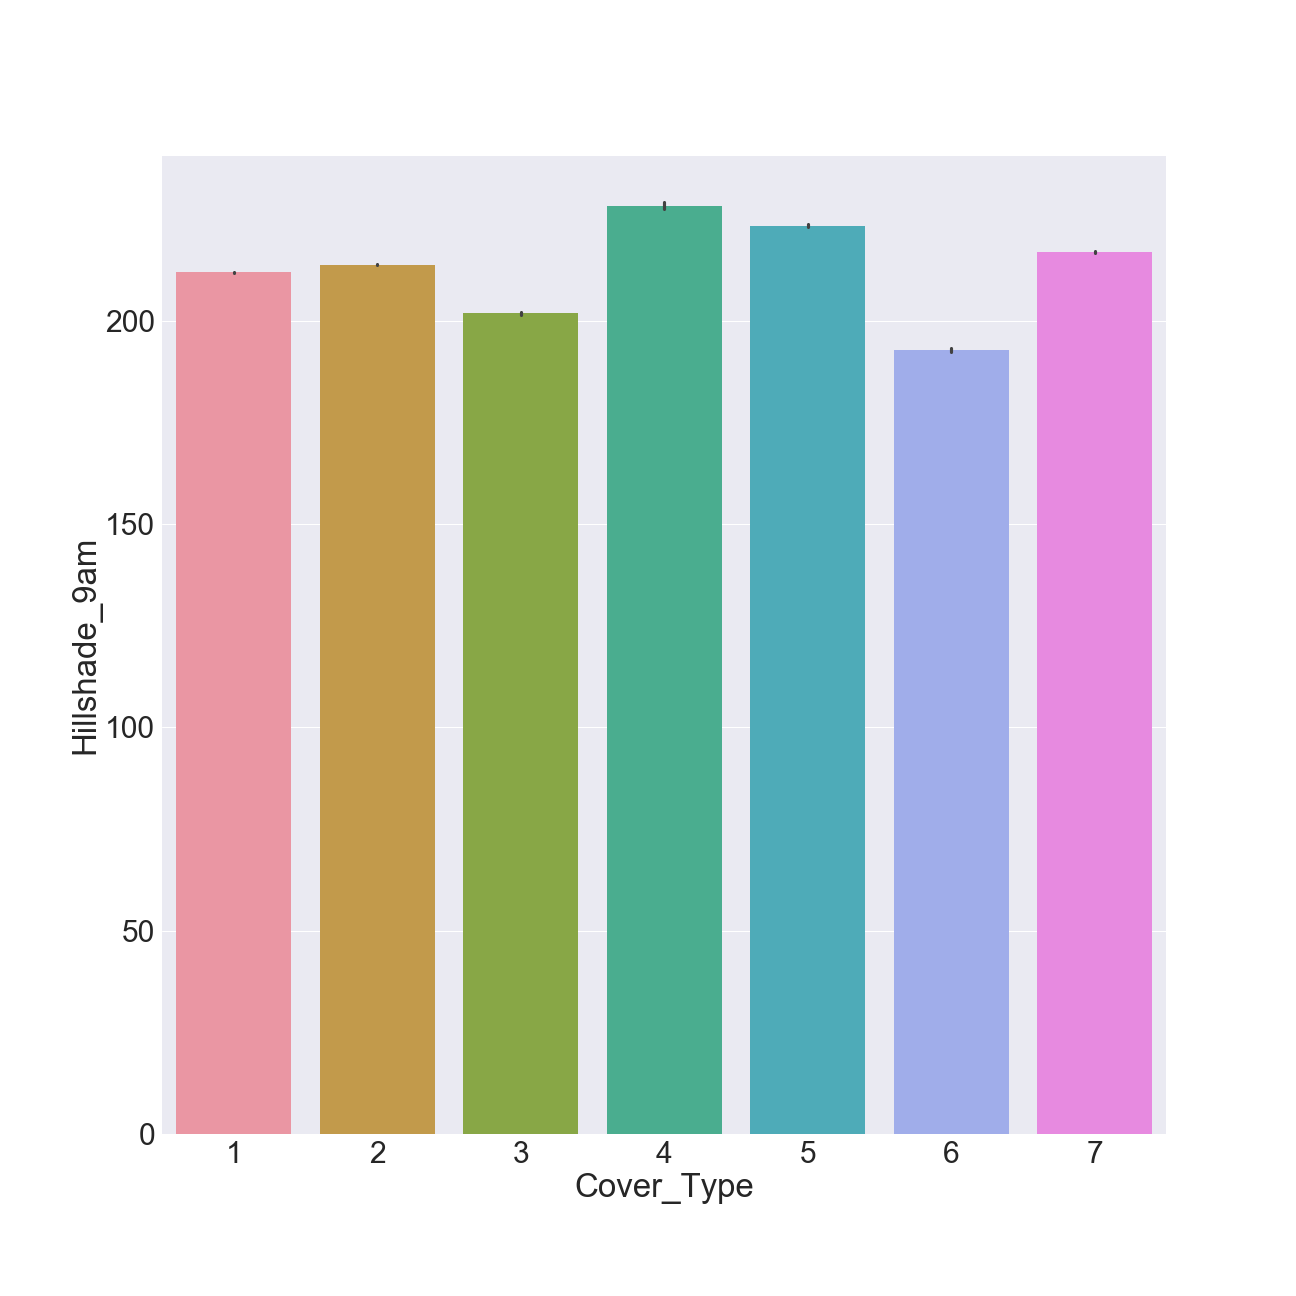
\includegraphics[width=0.5\textwidth]{Figures/Hillshade_9am_forest.png} &
%     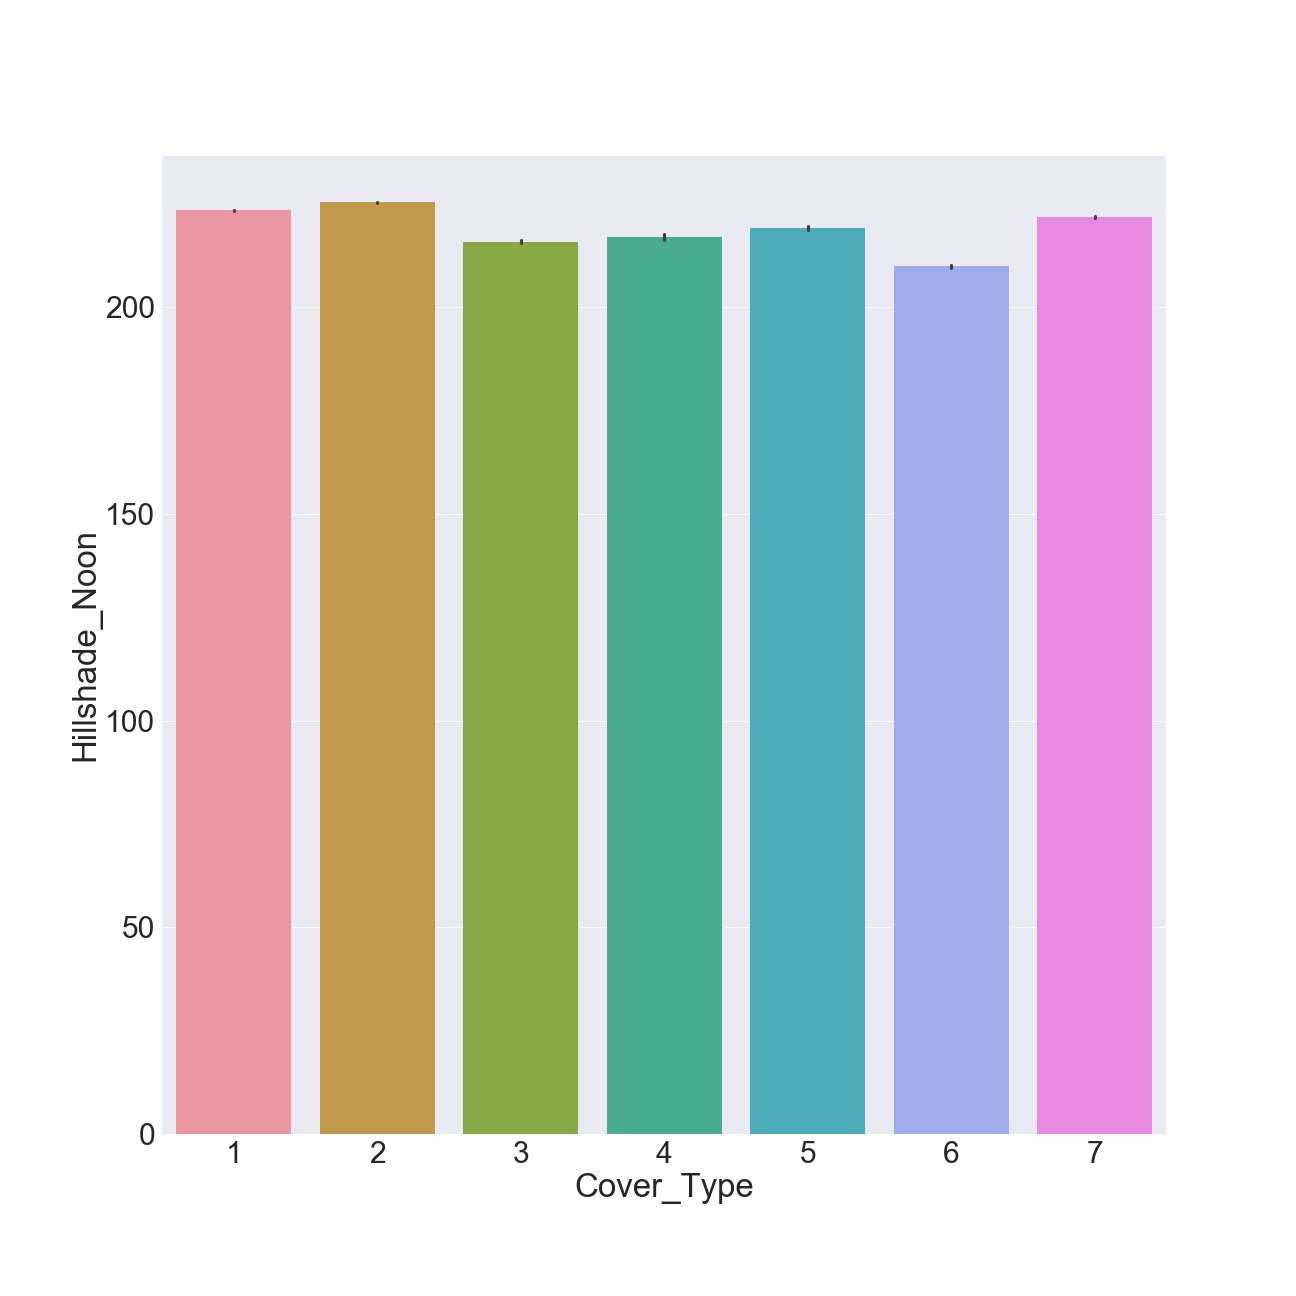
\includegraphics[width=0.5\textwidth]{Figures/Hillshade_Noon_forest.png} \\
%     (g)  & (h)  \\[6pt]
%     \end{tabular}

%     \begin{tabular}{cccc}
%     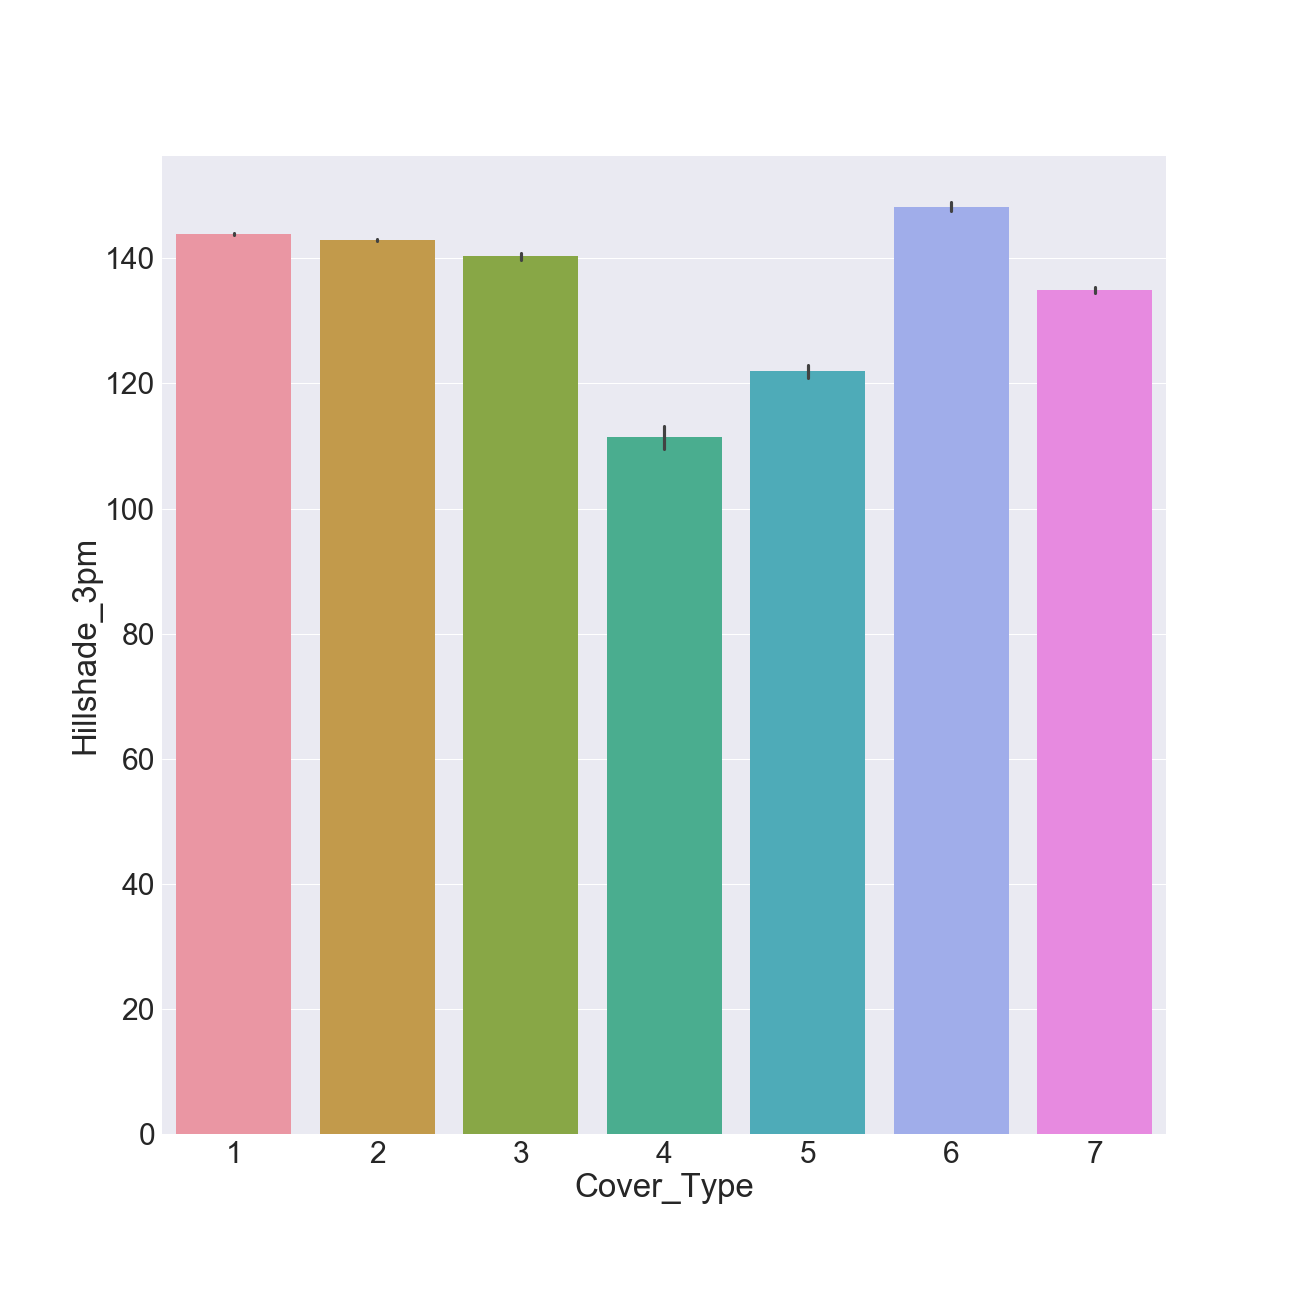
\includegraphics[width=0.5\textwidth]{Figures/Hillshade_3pm_forest.png} &
%     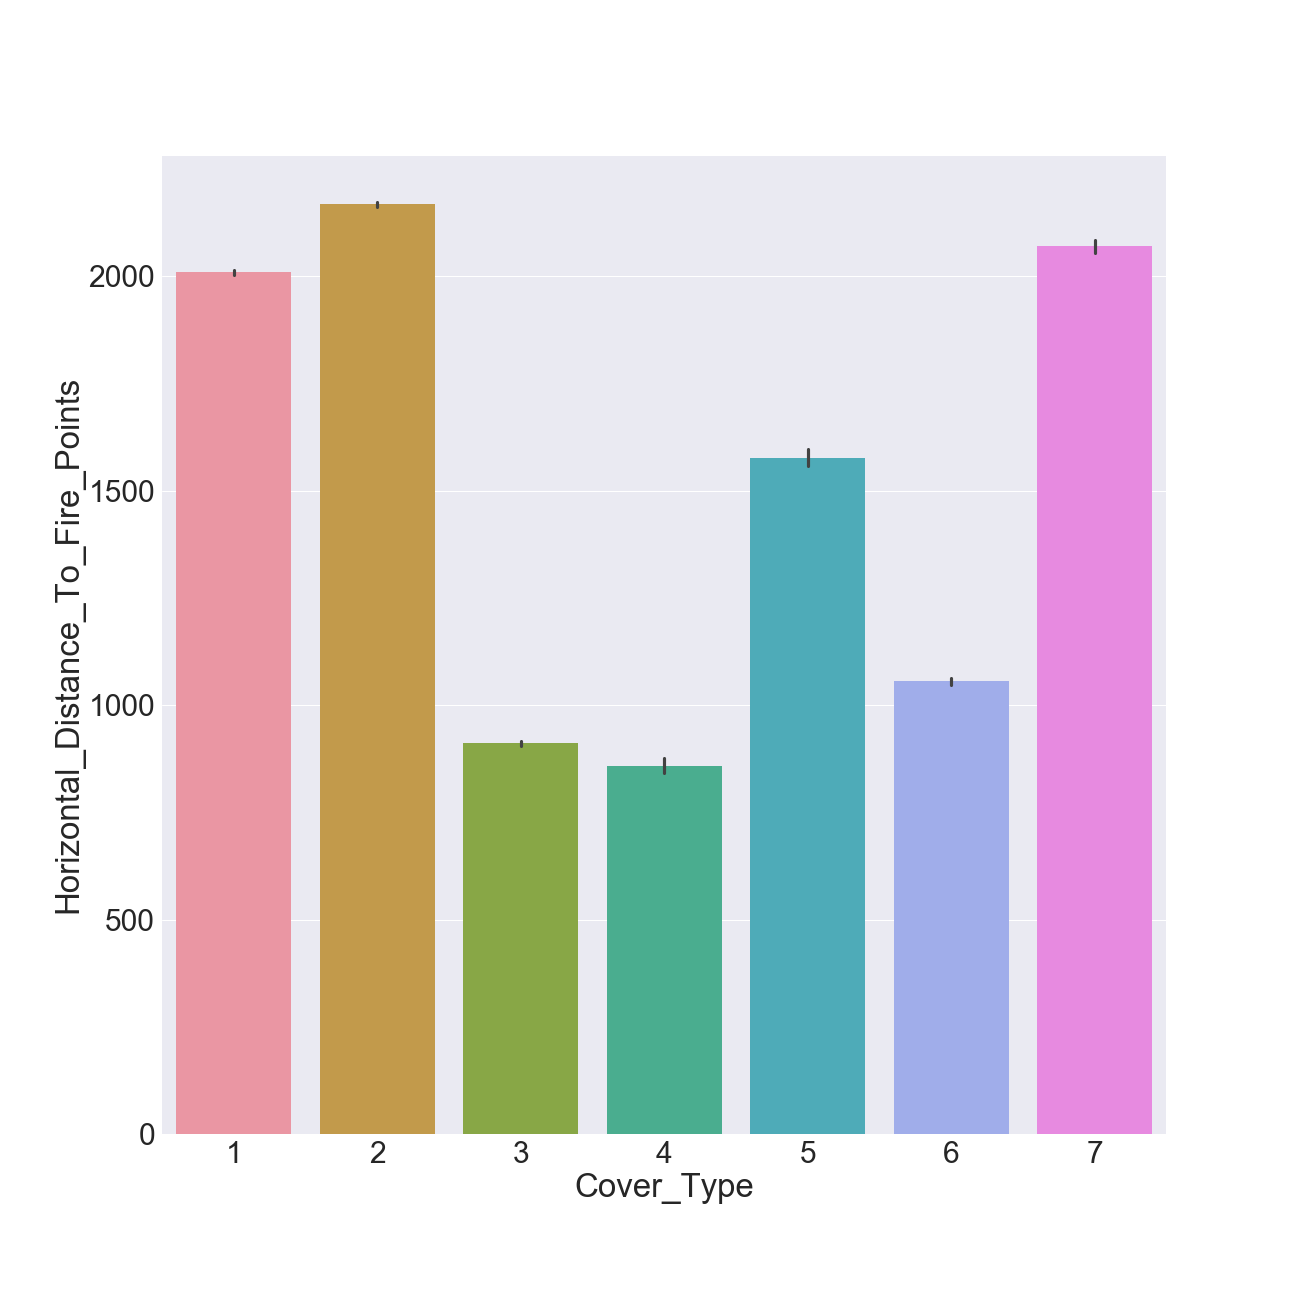
\includegraphics[width=0.5\textwidth]{Figures/Horizontal_Distance_To_Fire_Points_forest.png}\\
%     (i)  & (j)  \\[6pt]
%     \end{tabular}

% \caption{Cover type with respect to (a) elevation, (b) aspect, (c) slope, (d) horizontal distance to hydrology, (e) vertical distance to hydrology, (f) horizontal distance to roadways,  (g) hill-shade at 9am, (h) hill-shade at noon, (i) hill-shade at 3pm and (j) horizontal distance to fire points}
% \label{fig:wine_quality_2}
% \end{figure}

\begin{figure} [H]
    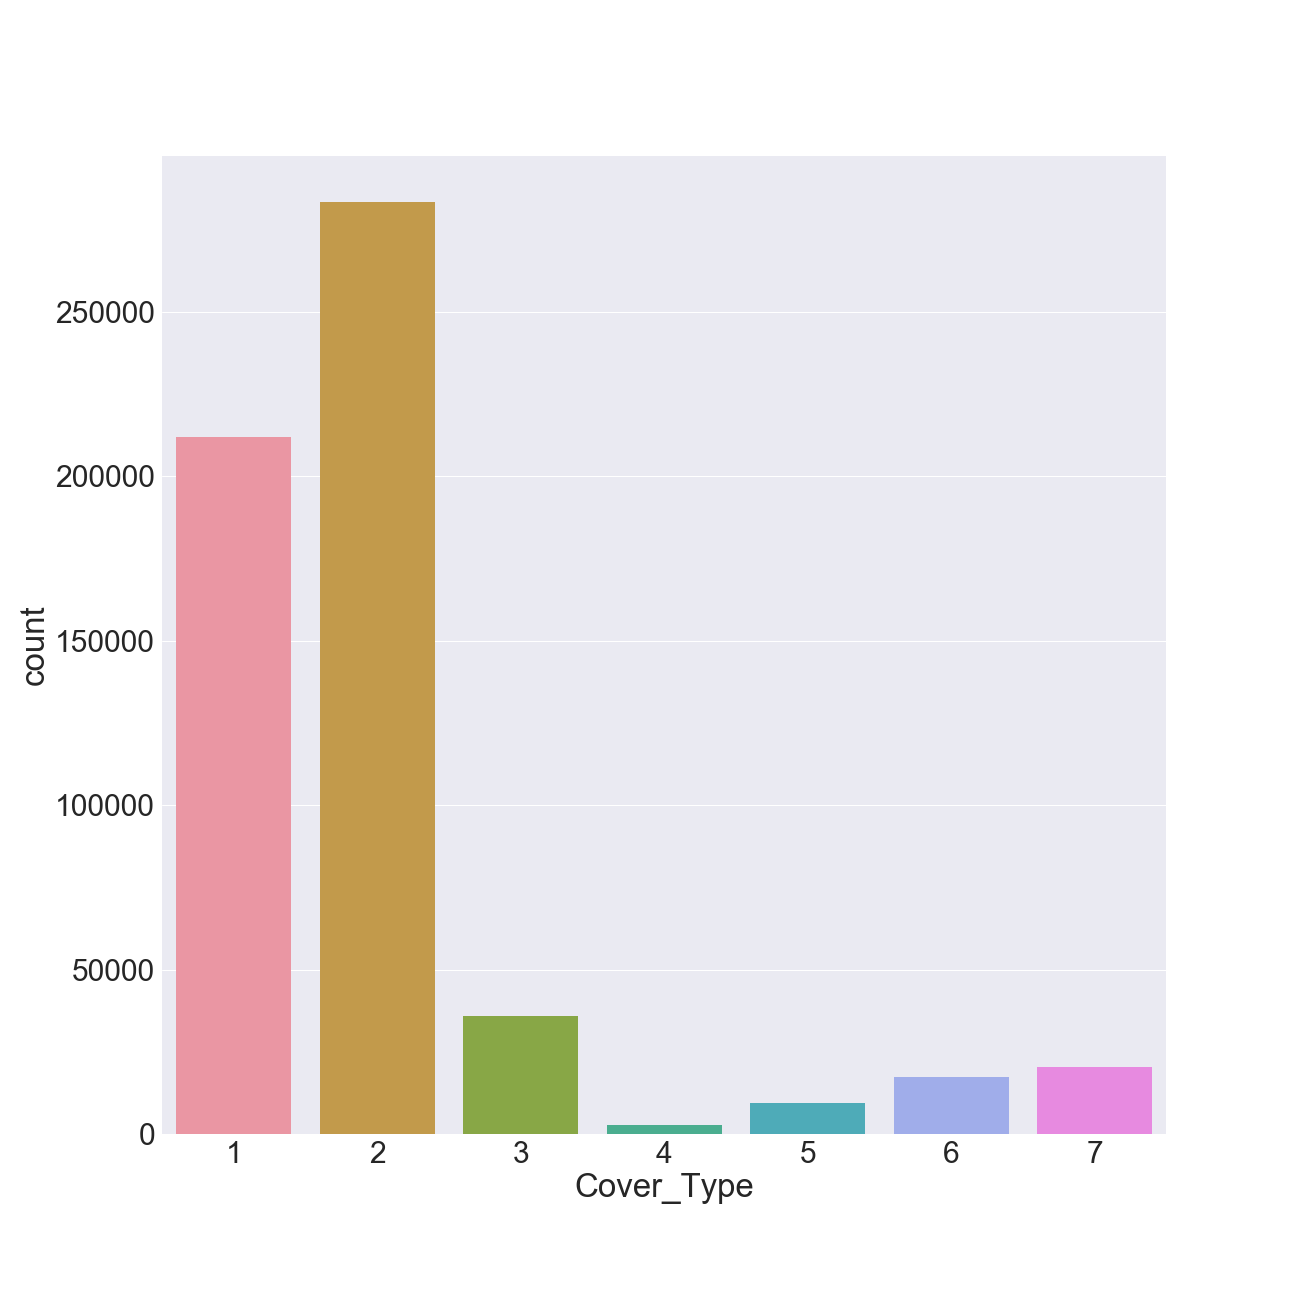
\includegraphics[width=1\textwidth]{Figures/instances_forest.png}
\caption{Distribution of the data}
\end{figure}
\label{fig:hist_wine}
\end{document}



\begin{comment}
\subsection{Support vector machine}
Support vector machine (SVM) is a supervised learning algorithm which try to find the separating hyperplane  with the largest margin in an N-dimensional space. To do so, this strong classifier try to find the support vectors which are the closest points to the separating hyperplane, and which provide the largest margin.\\

In the case where SVM is apply to linearly separable data, SVM with hard margin will be able to find the optimal hyperplane. In the other case where data is not linearly separable, SVM with soft margin can be use. This algorithm allows misclassified points by having an hyperparameter $C$ to control the "trade-off" between minimizing the training error and maximizing the margin\cite{Gar}. This "trade-off" can also be seen as a way to control the capacity of the model. In fact, the capacity of SVM decrease as the hyperparameter $C$ decrease (increase the margin size), because SVM allows more misclassified points. Another solution to non-linearly separable data is to transform this linear discriminant to a non-linear classifier by using kernel function. \\

Finally, SVM solve the quadratic objectif function and the following constraints
\begin{align*}
    \min_{\textbf{w},\xi}& \frac{1}{2}\|\textbf{w}\|^2 +C \sum_{i=1}^n\xi_i\\
        &s.t. \qquad (w^Tx_i+b)y_i\geq 1-\xi \qquad \forall i \in \{1,...,n\}\\
        &\hspace{2.7cm} \; \; \xi_i\geq 0 \hspace{1.3cm}\forall i \in \{1,...,n\}
\end{align*}

by using the Lagrange multipliers and the dual objectif function\cite{Zha}.


%Old comments - Decision tree
Figure \ref{fig:res_tree} in Appendix \ref{Appendice_Tree} show the performance ($F_1$ score and accuracy) on the training and test set of boosted and not boosted classifiers using decision trees. For the Wine Quality dataset, we can see that the maximum $F_1$-score (0.45) is obtained when the number of classifiers is equal to 32, yielding a gain of 0.11 over the single decision tree classifier. On the other hand, the accuracy is constant. We explain this by the fact that the wine dataset was highly unbalanced. Figure \ref{fig:hist_wine} show the distribution of the wine quality dataset. We can see that 2 of the classes represent more than half the data. We suspect that a small number of nodes was enough to maximized the accuracy, but we would have to investigate 
For the Forest Cover Type, boosting with 16 classifiers improved the performance by 0.07 compare to the non boosted classifiers. The performance seems to drop when the tree get smaller than a depth of 6. Its  For both datasets, the model is not overfitting the training data, even if the generalization is slightly better for the Forest Cover Type. 

 
 %For the Forest Cover Type classification, the boosted classifiers achieve better result than the single deeper classifier. While the overall relation is different, it is interesting to note that in the case of the Wine Quality classification the $F_1$-score was decreasing with the depth of the tree and the boosting seems to have leveled the score. On the other hand, for the Forest Cover Type classification decreasing the depth do not seems to affect the score as much. It is possible that we would have observed a similar pattern if we had compute the score for smaller trees. 
 
 %TODO: change accordingly to new results
% Logistic regression and Adaboost are quite similar, but they are computed differently. Logistic regression minimize the log-loss within a single optimization problem where Adaboost minimize the exponential loss iteratively and try to improve classification on the training set at each iteration \cite{Singh}. As we can see in Figure 3, it is interesting to observe that our baseline $F_1$-score clearly increase as the number of classifier in the boosted Logistic regression increase. This mean that as the residual error of a Logistic regression are not perfectly classify, we can use the information of these misclassified point and add a Logistic regression hyperplane to create a non-linear function with a better classification power without overfitting our training set.

%Figure \ref{fig:res_tree} in Appendix \ref{Appendice_Tree} show the performance ($F_1$ score and accuracy) on the training and test set of boosted and not boosted classifiers using decision trees. For the Wine Quality dataset, we can see that the maximum $F_1$-score (0.45) is obtained when the number of classifiers is equal to 32, yielding a gain of 0.11 over the single decision tree classifier. For the Forest Cover Type, boosting with 16 classifiers improved the performance by 0.07 compare to the non boosted classifiers. The performance seems to drop when the tree get smaller than a depth of 6. For both datasets, the model is not overfitting the training data, even if the generalization is slightly better for the Forest Cover Type. The classification accuracy is about 1.5 times higher for the Forest Cover Type, probably due to the fact that we balanced this data set. For both task, boosting the classifier improved the performance, showing that there can be value in boosting even when the total number of parameters in maintained constant.
\end{comment}




